\chapter{Theory and Foundations}
\label{ch:theory}

This chapter establishes the theoretical foundations that underpin the three
core contributions of this thesis: interpretable graph representations,
diffusion-based graph generation, and statistically grounded generative model
evaluation.
We begin by introducing the mathematical representation of graphs enriched with structural
and attribute information, toghether with the mathematical notation used
throughout the thesis. Fundamental concepts including permutation invariance,
matrix representations, and neighbourhood structures are presented to clarify
the computational and symmetry properties that distinguish graphs from
Euclidean data.

Building on this foundation, we review the principal paradigms of graph
representation learning, distinguishing between predefined
(data-independent) representations and learned (data-driven) embeddings.
This unified perspective situates graph kernels and neural models within a
common framework and highlights their complementary strengths.
We then survey modern deep generative models for graphs, with particular
emphasis on diffusion-based approaches and the challenges posed by the  
discrete structure of the graphs, permutation symmetry, and structural validity
constraints. Finally, we examine existing methodologies for evaluating generative models
and introduce learning-theoretic tools that enable statistically grounded and
reliable model comparison.Together, these components provide the conceptual, mathematical, and
methodological framework required for the developments presented in the
subsequent chapters.

\section{Graphs and Structured Data}


Graphs are a fundamental data structure for modeling relationships among entities
and arise naturally in a wide range of application domains, including social
networks~\citep{newman2003structure}, bioinformatics~\citep{borgwardt2005protein},
chemoinformatics~\citep{weininger1988smiles}, recommender systems~\citep{ying2018graph},
and cybersecurity~\citep{10.1145/310889.310919}. Unlike data embedded in regular
Euclidean domains such as images or sequences, graphs encode irregular,
non-Euclidean structures with variable neighbourhood sizes and complex
topologies~\citep{bronstein2017geometric}. This structural flexibility makes graphs
a powerful modeling formalism, but also introduces significant challenges for
representation, learning, generation, and evaluation.
\begin{definition}[Graph]
A (finite) graph is a tuple $G=(V,E)$, where
$V=\{v_1,\dots,v_n\}$ is a set of vertices and
$E \subseteq V \times V$ is a set of edges.
If $G$ is \emph{undirected}, edges are unordered pairs $\{u,v\}$; if
$G$ is \emph{directed}, edges are ordered pairs $(u,v)$.
\end{definition}
\begin{definition}[Graph isomorphism]
Two graphs $G=(V,E)$ and $G'=(V',E')$ are said to be \emph{isomorphic}
if there exists a bijection $\pi: V \to V'$ such that
\[
(u,v) \in E \iff (\pi(u),\pi(v)) \in E'.
\]
Graph isomorphism formalizes structural equivalence independently of
vertex ordering.
\end{definition}
\begin{figure}[h]
\centering
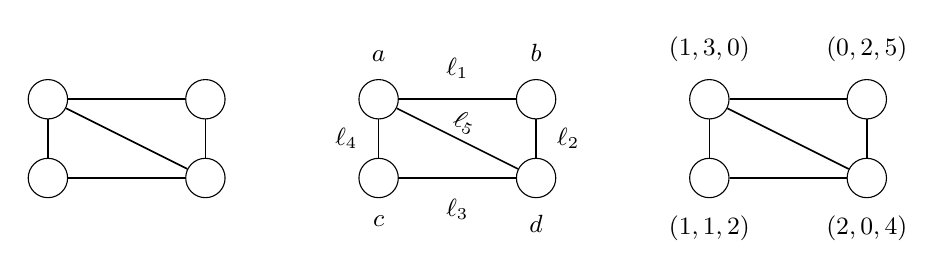
\begin{tikzpicture}[
  x=1cm,y=1cm,
  vnode/.style={circle,draw,minimum size=5mm,inner sep=0pt},
 % bigger circles
  edge/.style={line width=0.6pt},
  lab/.style={font=\small} % labels slightly larger
]

% ---------------- (a) undirected ----------------
\begin{scope}
  \node[vnode] (a1) at (0,1) {};
  \node[vnode] (b1) at (2,1) {};
  \node[vnode] (c1) at (2,0) {};
  \node[vnode] (d1) at (0,0) {};

  \draw[edge] (a1)--(b1);
  \draw[edge] (b1)--(c1);
  \draw[edge] (c1)--(d1);
  \draw[edge] (a1)--(c1);
      \draw[edge] (a1)--(d1);


  % no labels in (a), like your picture
\end{scope}

% ---------------- (b) labeled ----------------
\begin{scope}[xshift=4.2cm]
  \node[vnode] (a2) at (0,1) {};
  \node[vnode] (b2) at (2,1) {};
  \node[vnode] (c2) at (2,0) {};
  \node[vnode] (d2) at (0,0) {};

  % edges with labels
  \draw[edge] (a2)-- node[lab, above=4pt] {$\ell_1$} (b2);
  \draw[edge] (b2)-- node[lab, right=4pt] {$\ell_2$} (c2);
  \draw[edge] (c2)-- node[lab, below=4pt] {$\ell_3$} (d2);
  \draw[edge] (a2)-- node[lab, left=4pt] {$\ell_4$} (d2);
  \draw[edge] (a2)-- node[lab, sloped, above=-1pt] {$\ell_5$} (c2);

  % node labels OUTSIDE, farther away
  \node[lab, above=10pt] at (a2) {$a$};
  \node[lab, above=10pt] at (b2) {$b$};
  \node[lab, below=10pt] at (d2) {$c$};
  \node[lab, below=10pt] at (c2) {$d$};
\end{scope}
% ---------------- (c) real-valued attributed ----------------
\begin{scope}[xshift=8.4cm]
  \node[vnode] (a3) at (0,1) {};
  \node[vnode] (b3) at (2,1) {};
  \node[vnode] (c3) at (2,0) {};
  \node[vnode] (d3) at (0,0) {};

  \draw[edge] (a3)--(b3);
  \draw[edge] (b3)--(c3);
  \draw[edge] (c3)--(d3);
  \draw[edge] (a3)--(c3);
    \draw[edge] (a3)--(d3);


  % attribute labels OUTSIDE (like your picture) and farther away
  \node[lab, above=10pt] at (a3) {$(1,3,0)$};
  \node[lab, above=10pt] at (b3) {$(0,2,5)$};
  \node[lab, below=10pt] at (d3) {$(1,1,2)$};
  \node[lab, below=10pt] at (c3) {$(2,0,4)$};
\end{scope}

\end{tikzpicture}
\caption{(a) Unlabelled undirected graph. (b) Fully labeled graph (node and edge labels). (c) Attributed graph with real-valued node features.}
\label{fig:graph-types}
\end{figure}
In many real-world settings, graph structure alone is insufficient to fully
characterize the objects of interest. Nodes and edges are often associated with
additional information, such as atom types and charges in molecular graphs,
user profiles in social networks, or transaction metadata in cybersecurity
applications. This motivates the use of graphs augmented with label or attribute
information.

A graph whose vertices are assigned discrete labels is referred to as a
\emph{node-labeled} graph, while a graph whose edges carry labels is termed
\emph{edge-labeled}. When both vertices and edges are labeled, the graph is
\emph{discretely labeled}. Figure~\ref{fig:graph-types} illustrates several common
graph variants considered in this thesis, including an undirected graph, a fully
labeled graph, and a graph with real-valued node attributes.

\begin{definition}[Labeled graph]
A labeled graph is a graph $G=(V,E)$ equipped with a labeling function
$\ell: V \to \mathcal{L}$ and, optionally, an edge labeling function
$\ell_E: E \to \mathcal{L}_E$, where $\mathcal{L}$ and $\mathcal{L}_E$ are finite
sets of discrete labels.
\end{definition}
\footnote{Unless stated otherwise, all graphs considered in this thesis are simple graphs: they do not contain parallel edges or self-loops.}
In many applications, however, vertex and edge annotations are not restricted to
single discrete labels but take the form of feature vectors encoding multiple
categorical or real-valued properties. Graphs endowed with such vector-valued
annotations are known as \emph{attributed graphs}.

\begin{definition}[Attributed graph]
 An attributed graph is a graph $G=(V,E)$
equipped with node and, optionally, edge attributes. Let $d_x$ and $d_e$ denote
the dimensions of node and edge attributes, respectively. Node attributes are
specified by a function $x: V \to \mathbb{R}^{d_x}$, assigning a feature vector
$x_v$ to each node $v$, and edge attributes by a function
$e: E \to \mathbb{R}^{d_e}$, assigning a feature vector $e_{uv}$ to each edge
$(u,v)$. Attributes may be continuous or categorical.
\end{definition} 
We assume a fixed ordering of the vertex set $V=\{v_1,\dots,v_n\}$.
Under this ordering, the adjacency matrix provides a canonical matrix
representation of the graph structure and consists of $n$ rows and $n$ columns,
that is, $A\in\mathbb{R}^{n\times n}$.
For a vertex $v_i\in V$, its (open) neighbourhood is defined as
\[
N(v_i)=\{\,v_j\in V \mid (v_i,v_j)\in E\,\},
\]
that is, the set of vertices adjacent to $v_i$.
The degree of $v_i$ in $G$, denoted by $\deg_G(v_i)$, is the cardinality of its
neighbourhood, $\deg_G(v_i)=|N(v_i)|$.
These notions capture basic local structural properties and will be used
throughout this thesis.

\begin{definition}[Adjacency matrix]
Let $G=(V,E)$ be a graph with $|V|=n$ and a fixed vertex ordering.
The adjacency matrix $A\in\mathbb{R}^{n\times n}$ is defined by
$A_{ij}=1$ if $(v_i,v_j)\in E$ and $A_{ij}=0$ otherwise; for weighted graphs,
$A_{ij}$ may store an edge weight.
\end{definition}

\paragraph{Neighborhood and degree.}
For a vertex $v_i\in V$, the (open) neighbourhood is
\[
N(v_i)=\{\,v_j\in V \mid (v_i,v_j)\in E\,\}.
\]
The degree of $v_i$ in $G$, denoted $\deg(v_i)$, is the number of adjacent
vertices,
\[
\deg(v_i)=|N(v_i)|.
\]
The maximum degree of $G$ is $\deg^*=\max_{v\in V}\deg(v)$.
\paragraph{Laplacian matrix.}
Let $A$ be the adjacency matrix of $G=(V,E)$ and let
$D\in\mathbb{R}^{n\times n}$ be the diagonal degree matrix with
$D_{ii}=\sum_j A_{ij}$.
The (unnormalised) graph Laplacian is defined as
\[
L=D-A.
\]
\paragraph{Subgraphs.}
A graph $G'=(V',E')$ is a subgraph of $G=(V,E)$ if $V'\subseteq V$ and
$E'\subseteq E$.
Given a vertex subset $S\subseteq V$, the induced subgraph $G(S)$ is defined as
\[
\begin{aligned}
G(S) &= (S,E(S)), \\
E(S) &= \{(u,v)\in E \mid u,v\in S\}.
\end{aligned}
\]
\paragraph{Shortest paths and neighborhoods.}
Let $G=(V,E)$ be a graph and let $u,v\in V$ belong to the same connected
component. A \emph{path} between $u$ and $v$ is a sequence of adjacent vertices
connecting them. Among all such paths, there exists at least one with minimal
length, measured as the number of edges it contains; this follows from the
finiteness of the graph. The \emph{shortest-path distance} $d(u,v)$ is defined as
the length of such a shortest path. While multiple shortest paths may exist
between two vertices, their length is unique.

In weighted graphs, the distance $d(u,v)$ is defined as the minimum total weight
along any path connecting $u$ and $v$. Distances of this form are well defined
whenever edge weights are non-negative, and can be computed in polynomial time
using classical algorithms such as Dijkstra's algorithm \citep{dijkstra1959note}.


The notion of shortest-path distance induces a metric structure on each
connected component of the graph. This, in turn, gives rise to the concept of
local neighbourhoods. For a vertex $v \in V$ and radius $r \geq 0$, the radius-$r$ neighbourhood of $v$ is defined as
\[
N_r(v)=\{u \in V \mid d(u,v) \leq r\}.
\]
For unweighted graphs, this corresponds to the usual $r$-hop neighbourhood when
$r$ is an integer.
These neighborhoods capture increasingly large local regions of the graph and
play a central role in many graph representation, learning, and kernel-based
methods.
\paragraph{Permutation invariance and equivariance.}
A central challenge in learning on graphs is that vertex identities are
arbitrary: a relabeling of the vertices should not change the underlying
graph. Formally, let $n=|V|$ and let $\pi$ be a permutation of $\{1,\dots,n\}$.
We represent $\pi$ by its permutation matrix $P_\pi\in\{0,1\}^{n\times n}$.
If $A$ is the adjacency matrix under a given vertex ordering, then the same
graph under the relabeled ordering has adjacency matrix
\[
A^\pi \;=\; P_\pi A P_\pi^\top,
\]
and node features $X\in\mathbb{R}^{n\times d}$ transform as
\[
X^\pi \;=\; P_\pi X.
\]

\begin{definition}[Permutation invariance and equivariance]
Let $f$ be a function defined on graph representations.

\begin{itemize}
    \item $f$ is permutation invariant if
    \[
    f(A^\pi, X^\pi) = f(A,X)
    \quad \text{for all permutations } \pi .
    \]
    This property is required for graph-level outputs, such as graph embeddings
    or graph labels.

    \item $f$ is permutation equivariant if its output is node-wise,
    $f(A,X) \in \mathbb{R}^{n \times d'}$, and
    \[
    f(A^\pi, X^\pi) = P_\pi f(A,X)
    \quad \text{for all permutations } \pi .
    \]
    This property is required for node-level outputs, such as node embeddings
    or node-wise predictions, because relabelling the nodes should relabel the
    outputs in the same way.
\end{itemize}
\end{definition}

Most message-passing GNN layers are permutation equivariant at the node level,
and permutation-invariant graph representations are typically obtained by
applying a permutation-invariant readout (pooling) over node embeddings.
Graph Transformers similarly require structural encodings to inject relational
information while respecting these symmetry constraints.
\paragraph{Graph-level vs node-level tasks.}
Graph learning tasks can be categorized by prediction granularity.
In \emph{node-level tasks}, predictions are made for individual vertices
(e.g., node classification or link prediction), requiring permutation-equivariant
representations.
In \emph{graph-level tasks}, a single prediction is made for an entire graph
(e.g., molecular property prediction), requiring permutation-invariant
representations.
\section{Graph Representation Learning}
\label{sec:theory:representations}

The definitions introduced in the previous section describe graphs as abstract
combinatorial objects. In order to perform learning, generation, or evaluation
with graphs, however, these objects must be mapped to representations that are
amenable to computation. A \emph{graph representation} is therefore a mapping
from a graph (possibly with attributes) to a mathematical object on which
algorithms can operate (Figure~\ref{fig:graph-to-vector}).
% Preamble:
% \usepackage{tikz}
% \usetikzlibrary{arrows.meta,calc}
\begin{figure}[H]
\centering
\begin{tikzpicture}[
  >=Latex,
  vnode/.style={circle,draw,minimum size=4.2mm,inner sep=0pt},
  edge/.style={line width=0.7pt},
  lab/.style={font=\normalsize}
]

% ===================== LEFT: small graph =====================
% node coordinates chosen to resemble your screenshot
\node[vnode] (v1) at (0.0, 0.0) {$v_1$};
\node[vnode] (v2) at (1.2, 0.55) {$v_2$};
\node[vnode] (v3) at (2.4, 0.0) {$v_3$};
\node[vnode] (v4) at (1.2,-0.75) {$v_4$};
\node[vnode] (v5) at (1.2, 0.0) {$v_5$};

% edges (same connectivity feel)
\draw[edge] (v1)--(v2);
\draw[edge] (v2)--(v3);
\draw[edge] (v1)--(v5);
\draw[edge] (v5)--(v3);
\draw[edge] (v2)--(v5);
\draw[edge] (v5)--(v4);

% label under graph
\node[lab] at (1.2,-1.25) {graph $G=(V,E)$};

% ===================== MIDDLE: mapping arrow =====================
\draw[->,line width=0.9pt] (3.2,0.0) -- (6,0.0)
  node[midway,above=4pt,lab] {$\phi:\ \mathcal{G}\to\mathbb{R}^d$};

% ===================== RIGHT: bracketed vector =====================
% draw a tall stack of boxes
\def\x0{6.2}
\def\y0{-0.95}
\def\w{0.8}
\def\h{0.28}
\def\n{7}

% outer stack
\foreach \i in {0,...,6} {
  \draw[line width=0.5pt] (\x0,\y0+\i*\h) rectangle ++(\w,\h);
}

% light gray fills (varying lengths to look like "components")
\fill[black!20] (\x0,\y0+0*\h) rectangle ++(0.35,\h);
\fill[black!20] (\x0,\y0+1*\h) rectangle ++(0.55,\h);
\fill[black!20] (\x0,\y0+2*\h) rectangle ++(0.20,\h);
\fill[black!20] (\x0,\y0+3*\h) rectangle ++(0.65,\h);
\fill[black!20] (\x0,\y0+4*\h) rectangle ++(0.40,\h);
\fill[black!20] (\x0,\y0+5*\h) rectangle ++(0.25,\h);
\fill[black!20] (\x0,\y0+6*\h) rectangle ++(0.50,\h);

% bracket (left bracket only, like the screenshot)
% vertical
% \draw[line width=0.7pt] (\x0-0.18,\y0) -- (\x0-0.18,\y0+\n*\h);
% % rounded "hooks"
% \draw[line width=0.7pt,rounded corners=1.4mm]
%   (\x0-0.18,\y0+\n*\h) -- (\x0-0.34,\y0+\n*\h) -- (\x0-0.34,\y0+\n*\h-0.18);
% \draw[line width=0.7pt,rounded corners=1.4mm]
%   (\x0-0.18,\y0) -- (\x0-0.34,\y0) -- (\x0-0.34,\y0+0.18);

% text to the right
\node[lab,anchor=west] at (7,0.0) {$z=\phi(G)\in\mathbb{R}^d$};

\end{tikzpicture}
\caption{Mapping a graph $G$ to a fixed-dimensional vector representation $z=\phi(G)\in\mathbb{R}^d$.}
\label{fig:graph-to-vector}
\end{figure}

At a high level, graph representations can be broadly categorised according to
whether the mapping from graphs to representations is predefined or learned
from data (Figure~\ref{fig:graph_representation_taxonomy}).

\subsection{Structural encodings}
The most direct representations encode graph structure explicitly, for example
through adjacency matrices, degree matrices, or Laplacians. Such encodings
preserve the full combinatorial structure of the graph but depend on a fixed
vertex ordering. They can capture global structural information, but dense
matrix representations scale poorly: the adjacency matrix of a graph with
\(n=|V|\) vertices requires \(\mathcal{O}(n^2)\) memory
\citep{ji2025survey_graph_generation}. Models that operate directly on dense
\(n\times n\) adjacency representations are therefore usually restricted to
small graphs, such as molecular or protein structures, where the number of
vertices remains modest. For larger graph collections, matrix encodings are
more often used as intermediate representations or as building blocks for more
compact descriptions.
\begin{figure*}[h]
    \centering
    \makebox[\textwidth][l]{%
        
\includegraphics[
            width=1.0\textwidth,
            height=1.25\textwidth,
            keepaspectratio,
            trim=1.2cm 0 0cm 0,
            clip
        ]{images/graph_representation2.pdf}
    }
    \caption{
    Taxonomy of graph representation learning methods.
    Predefined (data-independent) representations specify a fixed mapping from
    graphs to features or similarities (e.g., explicit feature maps, graph
    kernels, or handcrafted structural descriptors), whereas learned
    representations are obtained through data-driven optimization, including
    matrix factorisation approaches and neural graph encoders.
    }
    \label{fig:graph_representation_taxonomy}
\end{figure*}
\subsection{Predefined (Data-Independent) Representations}
\label{sec:theory:predefined}

Predefined graph representations specify a fixed, deterministic mapping from a
graph to either a feature representation or a similarity measure. Depending on
the method, this mapping may be given explicitly as a feature map $\phi(G)$, or
implicitly via a kernel function $K(G_i,G_j)$ without constructing the feature
vector in closed form.

Such representations are defined independently of any downstream learning task
and are entirely determined by the chosen structural decomposition or feature
family. Their components typically correspond to well-defined substructures,
statistics, or patterns—such as walks, paths, neighborhoods, subgraphs, or
spectral quantities—capturing structural properties of the graph.

\subsubsection{Topological and Spectral Descriptors}

A classical class of predefined representations constructs
vector embeddings from hand-crafted structural descriptors.
These methods map a graph to a fixed dimensional feature vector
by computing statistics that summarize its topology,
such as degree-based quantities, shortest-path distances,
or cycle counts.
The resulting representation is deterministic and
independent of any learning objective. One of the earliest examples is the Wiener index
\citep{doi:10.1021/ja01193a005}, defined as the average
pairwise shortest-path distance in a graph.
Spectral embeddings constitute another important class:
the eigenvalues of the graph Laplacian encode global structural
information in a compact vector representation
\citep{brouwer2012spectra}.
Although non-isomorphic graphs may share identical spectra
\citep{WILSON20082833}, such embeddings remain useful in practice
and connect naturally to diffusion-based interpretations.
While computationally efficient, these explicit embeddings often
sacrifice structural expressivity.
This trade-off between efficiency and discriminative power
motivated the development of graph kernels, which aim to construct
richer feature representations while retaining computational
tractability.


\subsubsection{Graph Kernels}
\label{sec:theory:explicit}
A prominent class of predefined, data-independent representations is given by
\emph{graph kernels}, which define similarity functions between graphs that
correspond to inner products in a (possibly implicit) feature space
\citep{vishwanathan2010graph,kriege2020survey}. Through this construction, graph
kernels embed graphs into a vector space in a manner that is invariant to
permutations of vertex and edge orderings.
\begin{definition}[Explicit and implicit feature maps]
A kernel $k(x,y)$ admits an \emph{explicit feature map} if there exists a
finite-dimensional vector $\phi(x) \in \mathbb{R}^d$ such that
\[
k(x,y) = \phi(x)^\top \phi(y).
\]
It admits an \emph{implicit feature map} if the mapping $\phi$ exists but is
not constructed explicitly, often being infinite-dimensional, and kernel
values are computed directly via $k(x,y)$.
\end{definition}
\textbf{Kernel functions and Hilbert spaces.}
Let $\mathcal{X}$ be a non-empty set of objects.
A function $k:\mathcal{X}\times\mathcal{X}\to\mathbb{R}$ is called a
\emph{positive semidefinite (PSD) kernel} if, for any $N\in\mathbb{N}$ and any
$x_1,\dots,x_N\in\mathcal{X}$, the matrix
$K\in\mathbb{R}^{N\times N}$ defined by
\[
K_{ij}=k(x_i,x_j)
\]
is symmetric and positive semidefinite, i.e.,
\[
\sum_{i=1}^N \sum_{j=1}^N c_i c_j K_{ij} \ge 0
\quad \text{for all } c_1,\dots,c_N\in\mathbb{R}.
\]
The matrix $K$ is referred to as the \emph{Gram matrix} (or kernel matrix)
associated with $k$ and the inputs $\{x_i\}_{i=1}^N$. A fundamental result in kernel theory states that $k$ is a PSD kernel if and only
if there exists a Hilbert space $\mathcal{H}$ and a feature map
$\phi:\mathcal{X}\to\mathcal{H}$ such that
\[
k(x,y)=\langle \phi(x),\phi(y)\rangle_{\mathcal{H}}
\quad \text{for all } x,y\in\mathcal{X}.
\]
A Hilbert space is a complete inner-product space, meaning that every
\emph{Cauchy sequence} converges to a point within the space.
A sequence $(f_n)_{n\ge 1}$ is called Cauchy if, for every $\varepsilon>0$,
there exists a $N$ such that $\|f_n - f_m\| < \varepsilon$ for all $n,m \ge N$.
The Hilbert space associated with a kernel $k$ possesses the
\emph{reproducing property}
\[
f(x)=\langle f, k(x,\cdot)\rangle_{\mathcal{H}}
\quad \text{for all } f\in\mathcal{H},\, x\in\mathcal{X},
\]
and is therefore called a \emph{reproducing kernel Hilbert space} (RKHS)
\citep{Aronszajn1950TheoryOR}.

\textbf{Kernel methods.}
Kernel methods are learning algorithms that operate implicitly in an RKHS by
accessing data only through kernel evaluations, without explicitly constructing
the feature map $\phi$ \citep{scholkopf2001learning,soton259580}. This allows
kernel methods to be applied to structured input domains—such as strings,
trees, or graphs—that do not admit natural vector representations
\citep{gartner2003graph}.

\textbf{Graph kernels.}
Let $\mathcal{G}$ denote a set of graphs.
A \emph{graph kernel} is a kernel
$k:\mathcal{G}\times\mathcal{G}\to\mathbb{R}$ that measures similarity between
pairs of graphs. By definition, there exists a (possibly implicit) feature map
$\phi:\mathcal{G}\to\mathcal{H}$ into an RKHS such that
\[
k(G,H)=\langle \phi(G),\phi(H)\rangle_{\mathcal{H}}.
\]
Graph kernels therefore induce permutation-invariant
similarity functions and corresponding vector-space representations and enable the use of kernel-based learning algorithms
on graph-structured data.

\textbf{Levels of comparison.}
Graph representations can also be categorized according to the level at which
structure is encoded.
\emph{Node-level representations} associate each vertex with a descriptor that
captures local structure or attributes, and may later be aggregated to obtain
graph-level information. These representations may be explicit or learned, and
do not necessarily define kernels.
Classical kernel-based approaches typically operate at the \emph{graph level}. For example, random-walk kernels compare graphs by aggregating contributions from matching walks across the two graphs \citep{kashima2003marginalized,gartner2003graph}.
Such methods implicitly rely on node correspondences, but define similarity directly between entire graphs.
In contrast, many modern node-level representations are non-kernel methods.
Explicit examples include Weisfeiler--Lehman refinements and rooted subgraph features, while learned but non-neural approaches include random-walk–based embeddings such as DeepWalk \citep{perozzi2014deepwalk} and node2vec \citep{grover2016node2vec}.These methods produce vector representations of individual nodes without inducing a reproducing kernel
Hilbert space.

\textbf{R-convolution kernels.}
A general and widely used framework for defining kernels on structured objects
is given by \emph{R-convolution kernels} \citep{haussler1999}.
The central idea is to decompose a composite object, such as a graph, into a
collection of components—e.g., vertices, paths, or subgraphs—and to define the
kernel as an aggregation of similarities between pairs of components.

Formally, let $\mathcal{R}=\mathcal{R}_1\times\cdots\times\mathcal{R}_d$ denote a
space of components and let $\mathcal{R}^{-1}(X)$ be the set of valid
decompositions of an object $X$ into elements of $\mathcal{R}$. Given component
kernels $k_i$ on $\mathcal{R}_i$, the corresponding R-convolution kernel is
defined as
\[
k_{\mathrm{CV}}(X,Y)
=
\sum_{x\in \mathcal{R}^{-1}(X)}
\sum_{y\in \mathcal{R}^{-1}(Y)}
\prod_{i=1}^d k_i(x_i,y_i).
\]
If the component kernels are positive semidefinite and permutation invariant,
the resulting kernel is also positive semidefinite and invariant to vertex and
edge orderings, making this framework particularly well suited for graphs.

A known limitation of naive convolution kernels is diagonal dominance, where
highly specific components lead to excessive self-similarity. This observation
has motivated the development of weighted and structured decompositions in the
graph kernel literature \citep{kriege2020survey}.

The kernel proposed in this thesis belongs to the class of R-convolution kernels
and constructs an explicit, sparse feature representation based on structured
neighbourhood decompositions. This motivates Chapter~\ref{ch:nsppk}, where we develop a
kernel that preserves interpretability and scalability while directly supporting
continuous attributes without discretization.


\subsection{Substructure-Based Graph Kernels}

Table~\ref{tab:substructure-kernels} summarises representative
substructure-based graph kernels in terms of the graph substructures they compare,
their computational complexity, whether they admit explicit or implicit feature
maps, and their treatment of discrete and continuous attributes.
\begin{table}[h]
\centering
\caption{Overview of representative substructure-based graph kernels.}
\label{tab:substructure-kernels}
\resizebox{\textwidth}{!}{
\begin{tabular}{lccccc}
\toprule
Kernel & Substructure & Complexity & Feature map & Discrete labels & Continuous attributes \\
\midrule
Random Walk   & Walks                   & Cubic / high      & Implicit       & \checkmark & Partial \\
Shortest Path & Shortest paths           & Quadratic--cubic  & Explicit/implicit & \checkmark & Partial \\
Graphlet      & $k$-subgraphs            & Exponential in $k$ & Explicit       & \checkmark & Partial \\
WL Subtree    & Rooted subtrees          & Near-linear       & Explicit       & \checkmark & Limited \\
NSPDK         & Neighbourhood pairs      & Near-linear$^\ast$ & Explicit       & \checkmark & Discretised \\
NSPPK (ours)  & Neighbourhood + connector & Near-linear$^\ast$ & Explicit       & \checkmark & Direct \\
\bottomrule
\end{tabular}}
\end{table}

\subsubsection{Random Walk Kernels}
\label{sec:theory:rw_kernels}

Random walk kernels measure graph similarity by comparing
walks occurring in two graphs.
The central idea is to decompose each graph into the set of
its walks and aggregate similarities between pairs of walks.
Let $\mathcal{W}(G)$ denote the set of walks in a graph $G$.
A generic random-walk kernel can be written as
\[
k(G,G')
=
\sum_{\omega \in \mathcal{W}(G)}
\sum_{\omega' \in \mathcal{W}(G')}
k_{\mathrm{walk}}(\omega,\omega'),
\]
where $k_{\mathrm{walk}}$ compares the node and edge
label sequences induced by $\omega$ and $\omega'$.
In its simplest form, $k_{\mathrm{walk}}$ counts identical
label sequences.

\paragraph{Marginalized random-walk kernel.}
Kashima et al.~\citep{kashima2003marginalized}
introduced a probabilistic variant in which walks are
weighted by their probability under a random walk process.
The resulting kernel is
\[
k_{\mathrm{MRW}}(G,G')
=
\sum_{\omega \in \mathcal{W}(G)}
\sum_{\omega' \in \mathcal{W}(G')}
k_{\mathrm{walk}}(s(\omega), s(\omega'))
\, p(\omega \mid G)\,
p(\omega' \mid G'),
\]
where $p(\omega \mid G)$ is the probability of generating
walk $\omega$ in $G$.
This formulation allows the use of general positive definite
base kernels and can therefore incorporate continuous attributes.
Efficient implementations exploit the Kronecker structure of
the direct product graph and achieve
$\mathcal{O}(n^3)$ complexity for graphs with $n$ nodes
\citep{vishwanathan2010graph}.
Nevertheless, random-walk kernels remain computationally
expensive and are prone to \emph{tottering} effects,
where walks that repeatedly revisit nodes contribute little
discriminative information.
\subsubsection{Shortest-Path Kernel}
\label{sec:theory:sp_kernel}

The shortest-path kernel \citep{borgwardt2005shortest}
measures graph similarity by comparing the shortest paths
between all pairs of vertices in two graphs.
Instead of enumerating arbitrary walks, this approach first
transforms a graph $G=(V,E)$ into its \emph{shortest-path graph}
$S=(V,E_S)$, where an edge $(u,v)\in E_S$ exists whenever
$u$ and $v$ are connected in $G$, and its weight equals the
length of the shortest path between them.
Given two graphs $G$ and $G'$, the shortest-path kernel is defined as
\[
k_{\mathrm{SP}}(G,G')
=
\sum_{e \in E_S}
\sum_{e' \in E'_S}
k_{\mathrm{path}}(e,e'),
\]
where $k_{\mathrm{path}}$ compares shortest-path edges.
A common choice is
\[
k_{\mathrm{path}}(e,e')
=
k_{\mathrm{node}}(u,u')
\, k_{\mathrm{edge}}(e,e')
\, k_{\mathrm{node}}(v,v'),
\]
for edges $e=(u,v)$ and $e'=(u',v')$.
Here, node kernels compare endpoint labels,
while the edge kernel compares shortest-path lengths.
This formulation naturally supports both discrete
and continuous attributes.
Computing all-pairs shortest paths requires
$\mathcal{O}(n^3)$ time using Floyd–Warshall \citep{cormen2009introduction},
and the pairwise comparison of shortest-path edges
leads to a worst-case complexity of $\mathcal{O}(n^4)$.
If the path kernel admits an explicit $d$-dimensional
feature map, computation can be reduced to
$\mathcal{O}(n^2 d)$.
\subsubsection{Graphlet Kernel}
\label{sec:theory:graphlet_kernel}

The graphlet kernel \citep{shervashidze2009efficient}
compares graphs based on the distribution of small
induced subgraphs, called \emph{graphlets}.
Instead of enumerating arbitrary walks or paths,
this approach restricts attention to subgraphs
of a fixed size $k$.

Let $\mathcal{G}_k = \{g_1, \dots, g_{N_k}\}$ denote
the set of all (typically connected) graphlets of size $k$.
For a graph $G$, the \emph{$k$-spectrum} is defined as the vector
\[
\phi_{gd}(G) \in \mathbb{R}^{N_k},
\]
whose $i$-th entry counts the number of occurrences of graphlet
$g_i$ as an induced subgraph of $G$.
The graphlet kernel is then defined as the linear kernel
between these spectra:
\[
k_{\mathrm{GL}}(G,G')
=
\phi_{gd}(G)^\top \phi_{gd}(G').
\]
The spectra are typically normalised to account for
differences in graph size.

The main computational bottleneck is the enumeration
of all $k$-node subgraphs.
Since the number of possible graphlets grows
exponentially with $k$, practical implementations
restrict $k$ to small values (typically $k \in \{3,4,5\}$).
Under bounded degree assumptions, computation
scales as $\mathcal{O}(n deg^{k-1})$,
where $n$ is the number of nodes and $deg$ the maximum degree.

While graphlet kernels provide an explicit and
interpretable feature representation capturing
local structural motifs, they ignore larger-scale
structure and become computationally prohibitive
for increasing $k$.
Moreover, incorporating continuous node or edge
attributes typically requires additional extensions.
\subsubsection{Weisfeiler--Lehman Subtree Kernel}
\label{sec:theory:wl_subtree}

The Weisfeiler--Lehman (WL) subtree kernel
\citep{shervashidze2011weisfeiler}
is based on iterative refinement of node labels
inspired by the Weisfeiler--Lehman graph isomorphism test.
The key idea is to encode increasingly larger
rooted subtree patterns around each node through
repeated neighbourhood aggregation.

Let $G=(V,E)$ be a graph with initial node labels
$l_V(v)$.
At iteration $t=0$, we set
\[
l_V^{(0)}(v) = l_V(v).
\]
For $t \ge 0$, labels are updated according to
\[
l_V^{(t+1)}(v)
=
f\!\left(
l_V^{(t)}(v),
\big\{\, l_V^{(t)}(u) \mid u \in \mathcal{N}(v) \big\}
\right),
\]
where $\mathcal{N}(v)$ denotes the neighbors of $v$,
the multiset of neighbor labels is sorted,
and $f(\cdot)$ is an injective hashing function.
After $h$ iterations, node labels encode
rooted subtree structures of height $h$.

The WL subtree kernel constructs an explicit feature map
by counting label occurrences at each iteration.
Let $\Sigma^{(t)}$ denote the set of labels produced
at iteration $t$.
The feature representation of $G$ is
\[
\phi(G)
=
\big(
c(G,\sigma^{(0)}_1), \dots,
c(G,\sigma^{(h)}_j), \dots
\big),
\]
where $c(G,\sigma)$ counts the number of nodes
in $G$ assigned label $\sigma$.
The WL subtree kernel is then defined as the inner product
\[
k_{\mathrm{WL}}^{(h)}(G,G')
=
\langle \phi(G), \phi(G') \rangle.
\]

The relabeling procedure requires
$\mathcal{O}(h m)$ time for a graph with $m$ edges.
For fixed $h$, the method therefore scales
linearly in the size of the graph,
making it substantially more efficient
than random-walk or graphlet kernels.

In its standard form, the WL subtree kernel
is primarily designed for discrete node labels.
Continuous attributes typically require
discretization or additional adaptations.
The WL test also characterizes the expressive power of many graph neural
networks: message-passing GNNs are provably no more discriminative than the
1-WL isomorphism test in distinguishing non-isomorphic graphs.
\subsubsection{Neighborhood Subgraph Pairwise Distance Kernel (NSPDK)}
\label{sec:theory:nspdk}

The Neighborhood Subgraph Pairwise Distance Kernel (NSPDK)
\citep{costa2010fast}
extends substructure-based kernels by comparing
pairs of local neighbourhoods at controlled graph distances.
The key idea is to represent a graph through rooted
neighbourhood subgraphs and to assess similarity
between pairs of such neighborhoods.

Given a graph $G=(V,E)$ and a radius parameter $r$,
the $r$-neighbourhood of a node $v$ is defined as
\[
N^{(r)}(v)
=
\{ u \in V \mid d(u,v) \le r \},
\]
where $d(\cdot,\cdot)$ denotes shortest-path distance.
The corresponding induced subgraph is denoted
$G^{(r)}_v$.
In weighted graphs, $d(u,v)$ is defined via
edge-weight sums.

For fixed parameters $r$ and $d$,
NSPDK considers all pairs of nodes
$(v_1,v_2)$ such that $d(v_1,v_2)\le d$,
and compares the corresponding pairs of
rooted neighbourhood subgraphs.
The kernel is defined as
\[
k_{\mathrm{NSPDK}}(G,G')
=
\sum_{r,d}
\kappa_{r,d}(G,G'),
\]
where
\[
\kappa_{r,d}(G,G')
=
\sum_{\substack{(v_1,v_2) \in V^2 \\ d(v_1,v_2)\le d}}
\sum_{\substack{(v'_1,v'_2) \in {V'}^2 \\ d(v'_1,v'_2)\le d}}
k_\delta(G^{(r)}_{v_1},G'^{(r)}_{v'_1})
\, k_\delta(G^{(r)}_{v_2},G'^{(r)}_{v'_2}),
\]
and $k_\delta$ is typically a Dirac kernel on hashed
subgraph representations.

Subgraph representations are constructed via
canonical labeling and hashing.
For fixed small radii $r$ and distances $d$,
feature extraction scales near-linearly in the number
of edges.
This makes NSPDK substantially more scalable than
random-walk, shortest-path, or graphlet kernels.

NSPDK captures relational structure by pairing
local neighbourhoods at controlled distances,
thereby encoding both local and mid-range topology.
The kernel admits an explicit sparse feature map,
allowing efficient similarity computation via
dot products.
However, continuous attributes are typically
handled via discretization or hashing,
which may discard fine-grained information.



\subsection{Kernels for Node Attributed Graphs}

Table~\ref{tab:attributed-kernels} summarises representative kernels for
node-attributed graphs in terms of their core idea, support for continuous
attributes, reliance on discretisation, feature-map representation, and typical
computational complexity.

\begin{table}[h]
\centering
\caption{Overview of representative kernels for node-attributed graphs.}
\label{tab:attributed-kernels}
\resizebox{\textwidth}{!}{
\begin{tabular}{lccccc}
\toprule
Kernel & Core idea & Continuous attributes & Discretisation & Feature map & Complexity \\
\midrule
Propagation Kernel & Label diffusion & \checkmark & Often & Explicit & Near-linear \\
GraphHopper & Attributed shortest paths & \checkmark & No & Implicit & Quadratic \\
Multiscale Laplacian & Spectral hierarchy & \checkmark & No & Implicit & High \\
WWL Kernel & Optimal transport on WL distributions & \checkmark & No & Implicit & Cubic \\
Hash-based Kernels & Iterative hashing of substructures & \checkmark & Yes & Explicit & Near-linear \\
NSPPK (ours) & Neighbourhood + connector features & \checkmark & No & Explicit & Near-linear$^\ast$ \\
\bottomrule
\end{tabular}}
\end{table}

\subsubsection{Propagation Kernel}
\label{sec:theory:propagation_kernel}

The Propagation Kernel (PK) \citep{neumann2016propagation}
extends neighbourhood-based graph kernels to continuous node attributes.
It combines iterative feature diffusion with quantisation
to obtain an explicit feature representation.

Let $G=(V,E)$ be a graph with initial node attributes stored in matrix $P_0$,
where the $i$-th row corresponds to the attribute vector of node $v_i$.
At each iteration $t$, node attributes are updated via the propagation step
\[
P_{t+1} = D^{-1} A P_t,
\]
where $A$ is the adjacency matrix and $D$ is the diagonal degree matrix.
This corresponds to a random-walk diffusion of attributes across the graph.

Let $T$ denote the total number of propagation iterations.
After each propagation step, node attributes are quantised using a hashing
function that maps similar feature vectors to discrete bins.
Let $c_t(G,i)$ denote the number of nodes of graph $G$ assigned to bin $i$
at iteration $t$.
The feature map is defined as
\[
\phi(G)
=
\big(
c_0(G,1), \dots, c_T(G,n_T)
\big),
\]
and the propagation kernel is the linear kernel
\[
k(G,G') = \langle \phi(G), \phi(G') \rangle.
\]

The runtime scales as
$\mathcal{O}((T-1)m + Tn)$,
where $n$ and $m$ are the number of nodes and edges, respectively.
Thus, for fixed $T$, the method is near-linear in graph size.

The propagation kernel naturally handles continuous attributes and is
computationally efficient. However, it relies on discretisation of propagated
features, which may introduce sensitivity to quantisation choices and potential
information loss.

\subsubsection{GraphHopper Kernel}
\label{sec:theory:graphhopper}

The GraphHopper kernel \citep{feragen2013scalable}
extends the shortest-path kernel to graphs with
continuous node attributes.
While the classical shortest-path kernel relies
on exact matching of node labels and path lengths,
GraphHopper replaces these comparisons with
general node kernels, enabling the handling
of both discrete labels and continuous features.

Let $G=(V,E)$ be a graph with node labeling
function $\ell$.
For two nodes $v,u \in V$, let
$\pi_{vu}$ denote a shortest path between them.
Denote by $|\pi|$ the discrete length of the path
(number of vertices), and by $\pi(i)$ the $i$-th
vertex along the path.

The GraphHopper kernel is defined as a sum over
shortest-path pairs:
\[
k(G,G')
=
\sum_{\pi \in \mathcal{P}}
\sum_{\pi' \in \mathcal{P}'}
k_p(\pi,\pi'),
\]
where $\mathcal{P}$ and $\mathcal{P}'$ are the
sets of shortest paths in $G$ and $G'$ respectively.

The path kernel compares nodes encountered at
corresponding positions along paths:
\[
k_p(\pi,\pi')
=
\begin{cases}
\sum_{i=1}^{|\pi|}
k_n(\pi(i),\pi'(i)), & |\pi| = |\pi'|, \\
0, & \text{otherwise},
\end{cases}
\]
where $k_n$ is a kernel on node attributes
(e.g.\ Dirac for labels, linear or Gaussian for
continuous features).
This formulation can be rewritten as a weighted
sum of node kernels:
\[
k(G,G')
=
\sum_{v \in V}
\sum_{v' \in V'}
w(v,v')\, k_n(v,v'),
\]
where $w(v,v')$ counts how often $v$ and $v'$
appear at corresponding positions along shortest
paths of equal length.
Using efficient message-passing techniques,
the kernel can be computed in
\[
\mathcal{O}\!\left(n^2 (m + \log n + d + \delta^2)\right),
\]
where $n$ is the number of vertices,
$m$ the number of edges,
$d$ the attribute dimension,
and $\delta$ the graph diameter.
Thus, GraphHopper scales quadratically
in the number of vertices.

GraphHopper improves upon the classical
shortest-path kernel by naturally incorporating
continuous node attributes and avoiding
explicit enumeration of path pairs.
However, it remains computationally heavier
than neighbourhood-based kernels and
relies on implicit feature representations.


\subsubsection{Multiscale Laplacian Graph Kernel}
\label{sec:theory:multiscale_laplacian}

The Multiscale Laplacian Graph Kernel (MLGK)
\citep{kondor2016multiscalelaplaciangraphkernel}
compares graphs by modeling their structure
through Laplacian-based Gaussian distributions
at multiple scales.

Given an undirected graph $G=(V,E)$ with
Laplacian matrix $L$, the method interprets
the graph as defining a Gaussian distribution
$\mathcal{N}(0, (L+\eta I)^{-1})$,
where $\eta>0$ is a regularization constant.
Similarity between graphs is then defined
via a kernel between the corresponding
Gaussian distributions.

To achieve permutation invariance and
support graphs of different sizes,
vertices are first mapped to
local, permutation-invariant feature vectors.
Let $\phi(v)$ denote such a feature representation.
These vertex features induce a base kernel
\[
\kappa(v,u) = \phi(v)^\top \phi(u).
\]

The kernel is then lifted hierarchically:
for each vertex $v$, a nested sequence
of induced subgraphs
\[
v \in N_1(v) \subseteq \dots \subseteq N_{l_{\max}}(v)
\]
is constructed,
and Laplacian-based kernels are computed
between corresponding subgraphs across graphs.
The final multiscale kernel aggregates
these comparisons across levels.

Exact computation is expensive,
requiring repeated Laplacian inversions
with worst-case complexity up to
$\mathcal{O}(n^5 l_{\max})$.
Practical implementations employ
Nyström-type approximations and
low-rank projections to reduce cost,
but the method remains computationally heavy
compared to neighbourhood-based kernels.

MLGK captures structural information
at multiple scales and naturally supports
continuous node attributes.
However, it is implicit, computationally demanding,
and relies on spectral matrix operations,
which limit scalability in large graphs.


\subsubsection{Wasserstein Weisfeiler--Lehman (WWL) Kernel}
\label{sec:related:wwl}

The Wasserstein Weisfeiler--Lehman (WWL) kernel \citep{togninalli2019wasserstein}
addresses a key limitation of classical $R$-convolution graph kernels:
the aggregation of substructure similarities via simple summation or averaging,
which may discard distributional information.
Instead of comparing aggregated feature counts, WWL compares
\emph{distributions of node embeddings} using optimal transport.

\paragraph{WL-based node embeddings.}
Given a graph $G=(V,E)$, WWL first constructs node embeddings
using a Weisfeiler--Lehman (WL) propagation scheme.
For categorical labels, the standard WL refinement is applied:
\[
\ell^{(h+1)}(v)
=
\mathrm{hash}\!\left(
\ell^{(h)}(v),
\{\!\!\{\ell^{(h)}(u) : u \in \mathcal{N}(v)\}\!\!\}
\right),
\]
where $\{\!\!\{\cdot\}\!\!\}$ denotes a multiset, so repeated neighbour labels are
preserved during the aggregation.
For continuous attributes $a^{(0)}(v) \in \mathbb{R}^m$,
a continuous propagation step replaces hashing:
\[
a^{(h+1)}(v)
=
\frac{1}{2}
\left(
a^{(h)}(v)
+
\frac{1}{\deg(v)}
\sum_{u \in \mathcal{N}(v)}
w(v,u)\, a^{(h)}(u)
\right),
\]
where $w(v,u)$ denotes optional edge weights.
The final node embedding concatenates features across
iterations:
\[
f_H(G)
=
\mathrm{concat}\!\left(X_G^{(0)}, \dots, X_G^{(H)}\right),
\quad
f_H(G) \in \mathbb{R}^{|V| \times m(H+1)}.
\]

\paragraph{Graph Wasserstein distance.}
Given two graphs $G$ and $G'$, WWL defines a distance
between the sets of node embeddings via the
$1$-Wasserstein distance:
\[
D_W(G,G')
=
\min_{P \in \Gamma}
\langle P, M \rangle,
\]
where $M_{ij} = d(x_i, x'_j)$ is a ground distance
(Hamming for categorical features, Euclidean for continuous),
and $P$ is a transport plan with uniform marginals.
This compares graphs as \emph{distributions of nodes}
rather than via aggregated counts.

\paragraph{Kernel construction.}
The WWL kernel is obtained by exponentiating the
Wasserstein distance:
\[
k_{\mathrm{WWL}}(G,G')
=
\exp\!\big(-\lambda D_W(G,G')\big),
\]
yielding a Laplacian-type kernel.
For categorical features, the resulting kernel is
positive definite.
For continuous attributes, definiteness is not guaranteed
in general, and learning can be performed in a
Kreĭn space when necessary.

WWL retains the multiscale structural refinement of WL
while replacing histogram aggregation with optimal transport.
It naturally supports continuous node attributes and weighted edges,
and empirically improves performance on attributed graph benchmarks.
However, its main computational bottleneck lies in solving
the optimal transport problem, typically cubic in the number
of nodes.

\subsubsection{Hash-Based Kernels for Continuous Attributes}
\label{sec:theory:hash_kernels}
\citet{morris2016fasterkernelsgraphscontinuous} propose
\emph{hash graph kernels}, a general framework that converts continuous attributes into
discrete labels using randomized hashing, enabling any efficient discrete-label kernel to be
``lifted'' to attributed graphs.

Let $G=(V,E)$ be an attributed graph with node attributes
$a:V\to\mathbb{R}^d$ and let $\mathcal{H}=\{h:\mathbb{R}^d\to\mathbb{N}\}$ be a family of hash
functions. Sampling $h\sim\mathcal{H}$ induces a discretely labeled graph $h(G)$ by setting
$\ell(v)=h(a(v))$. Given a discrete base kernel $k_b$ (e.g.\ WL subtree or shortest-path),
the hash graph kernel averages kernel values over $I$ independent hashings:
\[
k_{\mathrm{HGK}}(G,H)
=
\frac{1}{I}\sum_{i=1}^{I} k_b\!\big(h_i(G),\,h_i(H)\big).
\]
When the base kernel admits an explicit feature map $\phi_b$, an explicit
representation for $k_{\mathrm{HGK}}$ is obtained by concatenating the
per-iteration feature vectors and normalising:
\[
\Phi(G)
=
\frac{1}{\sqrt{I}}
\Big(
\phi_b(h_1(G)) \oplus \cdots \oplus \phi_b(h_I(G))
\Big),
\qquad
k_{\mathrm{HGK}}(G,H)=\langle \Phi(G),\Phi(H)\rangle,
\]
where $\oplus$ denotes vector concatenation and $I$ is the number of hashing
iterations.
Thus, for fixed $I$, the hash kernel has essentially the same asymptotic running time as the
discrete base kernel (up to the linear factor $I$), while remaining applicable to continuous
attributes and benefiting from the scalability of explicit computation.

Hash-based kernels are attractive because they inherit (i) the speed and explicit feature maps
of discrete-label kernels and (ii) a principled way to incorporate continuous attributes via
randomized discretization. Their main limitation is that performance depends on the chosen
hash family and the number of iterations $I$: small $I$ can yield high variance, while large
$I$ increases computation. In addition, because attributes are ultimately reduced to discrete
codes, fine-grained similarity can be lost compared to methods that operate directly in the
continuous space. These trade-offs motivate approaches (such as our proposed kernel) that retain
explicit, scalable feature maps while integrating continuous attributes \emph{directly} rather
than through stochastic discretization.
\subsection{Learned representations}

In contrast to explicit representations, learned representations construct
graph embeddings through data-driven optimization. Rather than fixing a feature
map \(\phi\) a priori, these methods learn a parameterized mapping
\(\phi_\theta : \mathcal{G} \to \mathbb{R}^d\) whose parameters are optimized with
respect to a training objective, such as prediction accuracy, likelihood, or
reconstruction quality. Because learned representations are shaped jointly by the data distribution
and the optimization objective, they are typically more flexible than explicit
representations and can adapt to complex structural and attribute patterns.
This flexibility, however, comes at the cost of reduced interpretability,
increased sensitivity to dataset size and bias, and the need for careful
regularization and training. Learned graph representations can be broadly categorized into matrix
factorisation methods, random-walk-based approaches, proximity-preserving
deep embedding models, and deep neural network architectures. We review
these families in turn.

\subsubsection{ Matrix factorisation}
% in preamble
% \usepackage{graphicx} % for \resizebox
% \usepackage{tikz}
% \usetikzlibrary{positioning}

\begin{figure}[H]
\centering
\resizebox{\linewidth}{!}{%
\begin{tikzpicture}[
  font=\small,
  box/.style={
    rounded corners,
    draw=black!35,
    fill=gray!6,
    align=center,
    minimum width=4.0cm,
    minimum height=1.05cm,
    inner sep=5pt
  },
  arrow/.style={-Latex, thick}
]
\node[box] (G) {Graph $G=(V,E)$};

\node[box, right=1.6cm of G] (P)
{\textbf{Step 1: Proximity Matrix}\\
Adjacency  \ \textbar\  Laplacian \\
Higher-order proximity};

\node[box, right=1.6cm of P] (D)
{\textbf{Step 2: Decomposition}\\
Eigenvectors \ \textbar\  SVD\\
Low-rank factorisation};

\node[box, right=1.6cm of D] (Z)
{Node Embeddings\\
$Z \in \mathbb{R}^{|V|\times d}$};

\draw[arrow] (G) -- (P);
\draw[arrow] (P) -- (D);
\draw[arrow] (D) -- (Z);
\end{tikzpicture}%
}
\caption{General pipeline of matrix factorisation-based graph embedding methods.}
\label{fig:mf_pipeline}
\end{figure}

Matrix factorisation models constitute one of the earliest approaches to graph representation learning and have been widely used for node embedding tasks. These methods typically rely on singular value decomposition or related spectral techniques to project graph-derived matrices—such as adjacency, Laplacian, or transition matrices—into low-dimensional latent spaces.
In general, matrix factorisation methods can be expressed as learning
low-dimensional embeddings $Z \in \mathbb{R}^{|V|\times d}$ such that

\[
\Phi(Z) = \| M - ZZ^\top \|_F^2 + \lambda \mathcal{R}(Z),
\]

where $M$ denotes a graph-derived proximity matrix (e.g., adjacency,
Laplacian, or higher-order similarity matrix) and $\mathcal{R}(Z)$
is a regularization term. Under spectral formulations, this reduces
to computing the leading eigenvectors of $M$ or related operators.

One key advantage of matrix factorisation models is their relatively low training data requirement. Since embeddings are obtained through direct matrix decomposition rather than iterative parameter optimization, these methods are particularly effective in low-data regimes, where neural network--based approaches may suffer from overfitting. In addition, by operating on global graph representations such as the Laplacian matrix or transition matrix, matrix factorisation methods are able to capture proximity information between all pairs of nodes. Despite these advantages, matrix factorisation approaches also exhibit several limitations \citep{hoang2023graph}. In particular, their computational and memory complexity scale poorly with graph size \citep{cao2015grarep}, as decomposing large matrices becomes prohibitively expensive for graphs with millions of nodes. Moreover, matrix factorisation models struggle to handle incomplete or partially observed graphs, since missing or unseen values cannot be naturally incorporated into the decomposition process. As a result, these methods often lack generalization capability when graph data are sparse or evolving, motivating the development of neural network--based models that can better extrapolate to unseen nodes and edges \citep{dettmers2018convolutional}.While effective in capturing global structural information, the scalability limitations of matrix decomposition methods motivated the development of
sampling-based approaches that approximate structural proximity more efficiently.

\subsubsection{ Random-walk-based methods}
Although the main contributions of this thesis operate at the graph level,
node-level representation methods are reviewed because they provide the
building blocks for modern graph encoders and generative models.
Random-walk-based methods learn node representations by sampling a large number of paths from a graph and treating the resulting node sequences analogously to sentences in natural language. By applying probabilistic language models such as skip-gram, these methods preserve node proximity by maximizing the likelihood of observing neighboring vertices within a fixed context window \citep{Chen_2020}. A seminal approach in this category is DeepWalk, which performs uniform random walks to capture local neighbourhood structure and implicitly factorizes a node co-occurrence matrix \citep{perozzi2014deepwalk}. Building on this idea, node2vec introduces a biased random-walk strategy that interpolates between breadth-first and depth-first sampling, allowing the model to capture both community structure and structural equivalence in graphs \citep{grover2016node2vec}.Although computationally more scalable than full matrix decomposition,
these methods remain shallow and transductive, motivating deeper
neural architectures capable of learning hierarchical representations.

\subsubsection{Proximity-Preserving Deep Embedding Methods (Non-GNN)}

A class of deep embedding methods learns node representations by directly
preserving structural proximities in the graph using neural architectures,
without relying on sampled random walks or iterative message passing.
Unlike modern graph neural networks, these approaches do not perform
layer-wise neighbourhood aggregation; instead, they encode structural
information through reconstruction-based objectives.

LINE \citep{tang2015line} models both first-order proximity between directly
connected nodes and second-order proximity based on shared neighbourhood
structure, enabling scalable optimization on large graphs.
Structural Deep Network Embedding (SDNE) \citep{Wang2016StructuralDN}
extends this idea by employing a deep autoencoder that jointly preserves
local adjacency information and reconstructs higher-order neighbourhood
relationships through nonlinear transformations.
DNGR \citep{Cao_Lu_Xu_2016} captures more global structural information by
constructing a node similarity matrix via a random surfing process and
learning compact representations using a stacked denoising autoencoder.

In SDNE and DNGR, each node $v_i$ is associated with a high-dimensional
neighbourhood vector $s_i \in \mathbb{R}^{|V|}$ encoding its structural
similarity to all other nodes in the graph. An encoder network
$\mathrm{ENC}(\cdot)$ maps this vector to a low-dimensional embedding
$z_i = \mathrm{ENC}(s_i)$, while a decoder network
$\mathrm{DEC}(\cdot)$ attempts to reconstruct the original neighbourhood
vector:

\[
\mathrm{DEC}(z_i) \approx s_i.
\]

Thus, unlike other embedding methods such as DeepWalk and node2vec,
which learn embeddings via pairwise inner-product objectives over node
co-
occurrences, these approaches employ a unary decoder that reconstructs
the entire neighbourhood profile of each node. This reconstruction objective
incorporates structural information directly into the encoder.

However, the input dimensionality of the autoencoder scales with $|V|$,
which becomes computationally expensive for large graphs. Moreover,
since the architecture is tied to a fixed graph structure, these models
are strictly transductive: embeddings are learned for a single graph and
must be recomputed when new nodes or edges are introduced. Their limited
inductive capability and absence of iterative neighbourhood aggregation
motivated the development of graph neural network architectures capable
of generalizing to unseen nodes and evolving graph structures.


\subsubsection{Deep Neural Network Models}
\label{sec:theory:gnn}

Deep neural network–based models have emerged as a dominant paradigm for graph representation learning, driven by advances in deep learning and their ability to jointly model graph structure and node or edge attributes. These models extend classical embedding techniques by learning representations through parameterized neural architectures, enabling inductive generalization to unseen nodes and graphs. The most prominent class within this family is \emph{Graph Neural Networks} (GNNs), which learn node- or graph-level embeddings by iteratively aggregating and transforming information from local neighbourhoods.

\paragraph{Message passing formulation.}
\begin{figure}[H]
\centering
\begin{tikzpicture}[
  font=\small,
  vnode/.style={circle,draw,minimum size=6mm,inner sep=0pt},
  edge/.style={line width=0.7pt},
  msg/.style={-Latex, thick, draw=black!70},
  box/.style={rounded corners, draw=black!35, fill=gray!8, align=center}
]

% ================= LEFT: Graph =================
\node[vnode, fill=gray!20] (v) at (0,0) {$v$};
\node[vnode] (u1) at (-1.5,1) {$u_1$};
\node[vnode] (u2) at (-1.5,-1) {$u_2$};
\node[vnode] (u3) at (1.5,1) {$u_3$};
\node[vnode] (u4) at (1.5,-1) {$u_4$};

\draw[edge] (v)--(u1);
\draw[edge] (v)--(u2);
\draw[edge] (v)--(u3);
\draw[edge] (v)--(u4);

% ================= Messages =================
\draw[msg] (u1) -- (v);
\draw[msg] (u2) -- (v);
\draw[msg] (u3) -- (v);
\draw[msg] (u4) -- (v);

\node at (0,-2) {$\mathbf{m}_v^{(\ell)} = \mathrm{AGG}\{\psi(\mathbf{h}_u^{(\ell)})\}$};

% ================= RIGHT: Update =================
\node[box, right=4.2cm of v] (update)
{$\mathbf{h}_v^{(\ell+1)}
= \phi\!\left(\mathbf{h}_v^{(\ell)}, \mathbf{m}_v\right)$};

\draw[-Latex, thick] (v) -- (update);

\end{tikzpicture}
\caption{
Illustration of message passing in a GNN.
A target node $v$ aggregates transformed messages from its neighbors
$\mathcal{N}(v)$ and updates its representation via a learnable function.
}
\label{fig:gnn_message_passing}
\end{figure}
Most modern GNN architectures can be expressed within the \emph{message passing} framework. Let $G=(V,E)$ be a graph with node features $\mathbf{x}_v \in \mathbb{R}^{d_x}$ and, optionally, edge features $\mathbf{e}_{uv}\in\mathbb{R}^{d_e}$. A $L$-layer GNN maintains hidden states $\mathbf{h}_v^{(\ell)} \in \mathbb{R}^{d_\ell}$ for each node $v$, initialized as $\mathbf{h}_v^{(0)}=\mathbf{x}_v$. At layer $\ell$, node representations are updated via
\begin{align}
\mathbf{m}_v^{(\ell)}
&=
\mathrm{AGG}^{(\ell)}
\Big(\big\{
\psi^{(\ell)}(\mathbf{h}_v^{(\ell)}, \mathbf{h}_u^{(\ell)}, \mathbf{e}_{uv})
\ \big|\ u\in \mathcal{N}(v)
\big\}\Big),
\\
\mathbf{h}_v^{(\ell+1)}
&=
\phi^{(\ell)}\!\left(\mathbf{h}_v^{(\ell)}, \mathbf{m}_v^{(\ell)}\right),
\end{align}
where $\psi^{(\ell)}$ and $\phi^{(\ell)}$ are learnable functions and $\mathrm{AGG}^{(\ell)}$ is a permutation-invariant aggregation operator such as summation, mean pooling, max pooling, or attention-weighted aggregation. After $L$ layers, $\mathbf{h}_v^{(L)}$ encodes information from the $L$-hop neighbourhood of $v$.

This abstraction encompasses a wide range of architectures. Early GNN variants were based on recurrent neural networks, updating node states until convergence using shared parameters across layers \citep{li2016ggnn,selsam2019sat,tonshoff2023csp}. While recurrent GNNs capture both local and global dependencies, their weight-sharing mechanism limits multi-scale expressivity. To address these limitations, graph convolutional networks (GCNs) introduced layer-wise transformations with distinct parameters at each depth \citep{kipf2017semi}. Graph convolutional models can be broadly divided into spectral approa
ches, operating in the graph Fourier domain \citep{bruna2014spectral,defferrard2016cnn}, and spatial approaches, which implement localized message passing directly on the graph topology \citep{hamilton2017graphsage,velivckovic2018gat,xu2019powerful}.

More recent developments include attention-based GNNs, which assign adaptive importance weights to neighbors during aggregation \citep{velivckovic2018gat}, graph autoencoders such as GAE and VGAE that reconstruct graph structure from latent embeddings \citep{kipf2016vgae}, and graph transformer architectures that employ global self-attention mechanisms to capture long-range dependencies \citep{dwivedi2021graph,ying2021transformers,kreuzer2021rethinking,rampavsek2022recipe}. These transformer-based models relax strict locality constraints but typically require additional structural encodings to preserve permutation invariance.

\paragraph{Graph-level representations.}
For graph-focused tasks, node embeddings are aggregated into a single graph embedding using a permutation-invariant \emph{readout} function:
\[
\mathbf{z}_G
=
\mathrm{READOUT}\Big(\big\{\mathbf{h}_v^{(L)} \mid v\in V\big\}\Big),
\]
where $\mathrm{READOUT}$ may be global sum, mean, or max pooling, attention pooling, or hierarchical pooling mechanisms. The resulting representation $\mathbf{z}_G$ can then be used for graph classification, regression, or downstream prediction tasks.

\paragraph{Training objectives and inductive learning.}
GNNs can be trained under node, edge, or graph-level supervision. In node classification, a predictor $p_\theta(y_v \mid \mathbf{h}_v^{(L)})$ (e.g., softmax layer) is optimized on labeled nodes. In link prediction, a similarity function or multilayer perceptron operates on pairs $(\mathbf{h}_u^{(L)},\mathbf{h}_v^{(L)})$. In graph classification, predictions are made from $\mathbf{z}_G$.

A key methodological distinction concerns \emph{transductive} versus \emph{inductive} settings. In transductive learning, all nodes are observed during training but only a subset is labeled. In inductive learning, the model must generalize to previously unseen nodes or entirely new graphs. Because GNNs learn local aggregation rules rather than node-specific parameters, many architectures naturally support inductive generalization.



Despite their expressive power, deep neural network–based graph models face several well-documented challenges. Increasing depth may lead to \emph{over-smoothing}, where node representations become indistinguishable \citep{oono2019graph}. Scalability can be limited by neighbourhood expansion and memory constraints when operating on large graphs. Moreover, learned embeddings may be sensitive to noisy edges, distributional shifts, or adversarial perturbations. 
These limitations motivate ongoing research into regularization strategies, sampling-based training, architectural refinements, and hybrid approaches that combine learned and explicit representations.
\paragraph{Graph Transformers and Global Attention.}
While message-passing GNNs aggregate information locally through iterative
neighbourhood expansion, Transformer architectures replace localized aggregation
with global self-attention mechanisms.
Given a set of node embeddings
$X = [\mathbf{x}_1,\dots,\mathbf{x}_n] \in \mathbb{R}^{n\times d}$,
a self-attention layer computes updated representations by
\begin{align}
\mathbf{a}_{ij}
&=
\mathrm{softmax}_j\!\left(
\frac{(\mathbf{Q}\mathbf{x}_i)^\top (\mathbf{K}\mathbf{x}_j)}
{\sqrt{d}}
\right),
\\
\hat{\mathbf{x}}_i
&=
\sum_{j=1}^{n}
\mathbf{a}_{ij}\, \mathbf{V}\mathbf{x}_j,
\end{align}
where $\mathbf{Q},\mathbf{K},\mathbf{V}$ are learnable projections.
Multi-head attention computes several such attention maps in parallel and
concatenates their outputs.
Unlike message passing, self-attention allows each node to directly attend to
all other nodes in a single layer, thereby alleviating long-range dependency
and over-squashing issues associated with deep neighbourhood aggregation.

However, self-attention without positional encodings is permutation equivariant and does not encode explicit relational structure.
Graph Transformer variants therefore incorporate structural inductive bias
through positional or structural encodings, such as Laplacian eigenvectors,
shortest-path distances, random-walk features, or edge-type encodings.
These encodings provide relational context analogous to positional encodings
in sequence models while preserving permutation invariance.
Empirically, graph Transformers often outperform conventional GNNs on tasks
requiring global reasoning or complex attribute interactions
\citep{dwivedi2021graph,ying2021transformers,kreuzer2021rethinking,rampavsek2022recipe}.
Nevertheless, their quadratic attention cost in the number of nodes and the
need for carefully designed structural encodings pose scalability challenges,

\subsection{Kernels versus GNN embeddings}

Graph kernels and graph embeddings reflect two complementary perspectives
on representation learning for structured data.
Kernels emphasize pairwise comparison by defining an explicit similarity
function $k(G_i,G_j)$, and are naturally suited to similarity assessment,
ranking, and kernel-based classification, particularly in small-sample
regimes. Because they rely on deterministic feature maps and convex
optimization procedures, kernel methods often provide stronger
reproducibility guarantees and greater interpretability than deep
end-to-end models.
Embedding-based methods, in contrast, produce vector representations of
individual graphs or nodes through parameterized models trained on
task-specific objectives. These approaches are well suited for large-scale
prediction, representation transfer, and generative modeling pipelines,
where joint optimization and inductive generalization are desirable.Importantly, the choice between kernels and learned embeddings is not
merely architectural but methodological. Kernels offer explicit control
over structural inductive bias and feature construction, whereas neural
embeddings trade explicit structure for adaptive expressivity.
These differences have important implications for scalability,
interpretability, statistical robustness, and evaluation —
issues that are central to the contributions developed in this thesis.


\section{Deep Generative Models for Graphs}
\label{sec:related:generation}

\begin{figure}[H]
    \centering
    \hspace*{-1.4cm}
    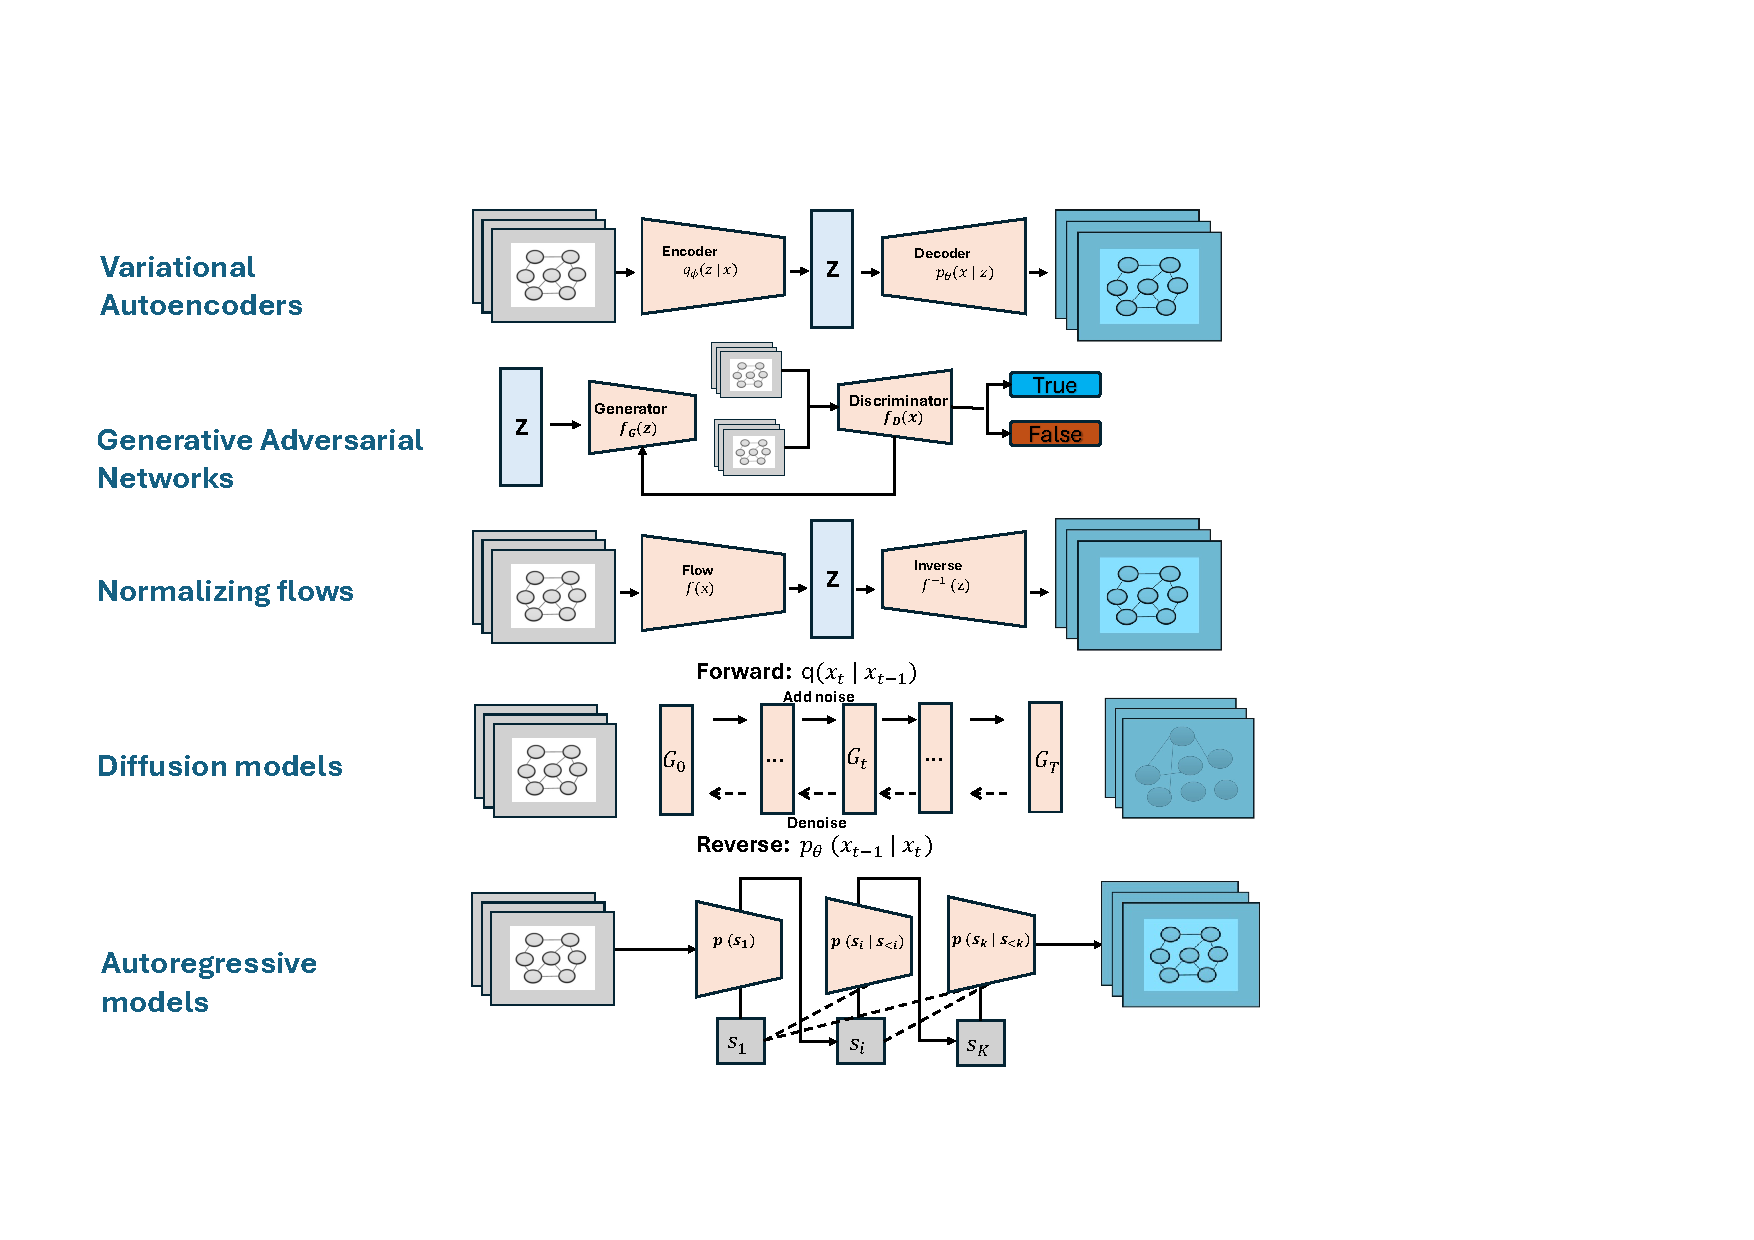
\includegraphics[width=1.5\textwidth]{images/graph_models.pdf}
    \caption{
    Overview of major deep generative modeling paradigms for graphs.
    \textbf{Variational Autoencoders (VAEs)} learn a probabilistic encoder 
    $q_{\phi}(z \mid G)$ and decoder $p_{\theta}(G \mid z)$ to model graph distributions 
    via latent variable inference.
    \textbf{Generative Adversarial Networks (GANs)} train a generator and discriminator 
    in an adversarial min--max game to implicitly approximate the graph data distribution.
    \textbf{Normalizing Flows} construct an invertible mapping between graphs and latent variables, 
    enabling exact likelihood computation via the change-of-variables formula.
    \textbf{Diffusion models} progressively corrupt graphs through a forward noising process 
    and learn a reverse denoising process $p_{\theta}(x_{t-1} \mid x_t)$.
    \textbf{Autoregressive models} factorize the graph likelihood according to the chain rule, 
    generating graph components sequentially as 
    $p(G)=\prod_{i} p(s_i \mid s_{<i})$.
    }
    \label{fig:graph_generative_taxonomy}
\end{figure}
While the preceding discussion focused on how graphs are represented for
downstream predictive tasks, an equally important question concerns how
graphs themselves can be generated. In contrast to representation learning,
graph generation requires modeling the full joint distribution over
combinatorial structures and attributes, posing additional challenges
related to permutation invariance, validity constraints, and scalability.
We therefore now turn to deep generative models for graphs.

\paragraph{Autoregressive Models.}

Autoregressive generative models construct complex data distributions by
factorizing the joint probability of a graph into a product of conditional
distributions using the chain rule of probability.
Given a sequential representation $S = (s_1, \dots, s_K)$ derived from a graph
$G$, the model generates components one step at a time according to
\[
p(G) = \prod_{i=1}^{K} p(s_i \mid s_{<i}),
\]
where $s_{<i}$ denotes the previously generated components.
In the context of graphs, such sequential representations may correspond to
node lists, edge lists, motif sequences, or traversal-based encodings.
Autoregressive approaches therefore generate graphs incrementally, deciding at
each step how to extend the current partial structure.
Representative methods include GraphRNN \citep{graph}, which generates
nodes and their adjacency vectors sequentially, NetGAN \citep{bojchevski2018netgan},
which models random walks as sequences, BiGG \citep{dai2020scalable}, which adopts
a tree-structured edge-generation process, and more recent large language
model–inspired approaches that tokenize graph structures into reversible
sequences \citep{zhao2023graphgpt}.
While autoregressive models provide flexible likelihood-based generation and
naturally handle variable-sized graphs, they often suffer from sequential
sampling inefficiency and sensitivity to the chosen graph ordering.
\paragraph{Variational Autoencoders (VAEs).}
Variational Autoencoders (VAEs) constitute one of the earliest
likelihood-based deep generative modeling paradigms.
They introduce a latent variable model in which observed data
$G$ is generated from a continuous latent representation
$z \sim p(z)$ through a decoder $p_\theta(G \mid z)$.
Because the true posterior $p_\theta(z \mid G)$ is generally intractable,
VAEs employ a variational approximation
$q_\phi(z \mid G)$ and optimize a lower bound on the log-likelihood
via stochastic gradient methods \citep{kingma2013auto,rezende2014stochastic}.
In the context of graph-structured data, VAEs have been adapted
by parameterizing both the encoder and decoder using graph neural
networks. The encoder $q_\phi(z \mid G)$ maps graphs into
continuous latent embeddings, while the decoder $p_\theta(G \mid z)$
reconstructs adjacency structures and node attributes from latent samples.
Representative approaches include the Variational Graph Autoencoder (VGAE)
\citep{kipf2016vgae} and subsequent extensions for structured
graph generation \citep{simonovsky2018graphvae}.

\paragraph{Generative Adversarial Networks (GANs).}

Generative Adversarial Networks (GANs) are implicit generative
models that learn the data distribution through an adversarial
min--max game between two neural networks: a generator
$f_G$ and a discriminator $f_D$.
The generator aims to synthesize graphs that resemble samples
from the true data distribution, while the discriminator seeks
to distinguish generated graphs from real ones.
The adversarial objective can be written as
\[
\min_{f_G} \max_{f_D}
\;
\mathbb{E}_{G \sim p_{\text{data}}}
[\log f_D(G)]
+
\mathbb{E}_{z \sim p(z)}
[\log (1 - f_D(f_G(z)))] ,
\]
where $z$ is drawn from a simple latent prior distribution.

Extending GANs to graph generation introduces additional
challenges due to the discrete and combinatorial nature of
graph structures.
Since gradients cannot be directly propagated through discrete
sampling operations, many graph GAN models rely on
continuous relaxations or reinforcement learning techniques
to enable optimization.
Representative approaches include GraphGAN
\citep{wang2018graphgan}, which models vertex connectivity
via adversarial learning; NetGAN \citep{bojchevski2018netgan},
which generates graphs through biased random walks and
optimizes a Wasserstein adversarial objective; and MolGAN
\citep{de2018molgan}, which integrates adversarial training
with reinforcement learning for molecular graph generation.
Despite their flexibility and ability to produce high-quality
samples, GAN-based graph models often suffer from
training instability, convergence sensitivity, and mode collapse,
which may limit structural diversity and scalability.

\paragraph{Normalizing Flows.}

Normalizing flow models learn an explicit density over data by
composing a sequence of invertible transformations
$f = f_L \circ \dots \circ f_1$ that map graph representations
(e.g., adjacency tensors or edge features) to latent variables
$z$ drawn from a simple base distribution.
Under the change-of-variables formula, the likelihood of a graph
sample $G$ can be computed exactly as
\[
\log p(G)
=
\log p(z)
+
\sum_{\ell=1}^{L}
\log \left| \det
\frac{\partial f_\ell}{\partial h_{\ell-1}}
\right|,
\]
where the determinant of the Jacobian quantifies how each
invertible transformation alters local volume in the data space.
The bijective structure of $f$ enables tractable density estimation
and exact sampling via the inverse mapping $f^{-1}(z)$.In graph generation, early flow-based approaches such as
MoFlow \citep{zang2020moflow}
adopt a two-stage generation procedure in which molecular
bond structures are generated using a Glow-style continuous flow,
followed by conditional generation of atom types.
GraphDF \citep{lu2022graphdf} extends this paradigm by
introducing discrete normalizing flows based on invertible
modulo-shift transformations, thereby avoiding continuous
relaxations and achieving exact invertibility over discrete
graph variables. GGFlow \citep{hou2024improving} combines
discrete flow matching with optimal transport and an
edge-augmented graph transformer to better model complex
bond interactions in molecular graphs. While normalizing flows provide principled density modeling
with exact likelihood evaluation, the requirement of strict
invertibility constrains architectural flexibility and may limit
their ability to capture large-scale, global node–edge
dependencies characteristic of complex graph topology.


\paragraph{Limitations}

Despite substantial advances, existing deep generative models
continue to face fundamental challenges when applied to
graph-structured data.

Likelihood-based approaches such as VAEs require
explicit or implicit handling of permutation invariance.
In practice, this often entails costly graph-matching procedures
or approximate estimation over possible node alignments,
which can significantly increase computational complexity
and introduce approximation bias \citep{simonovsky2018graphvae}.
Adversarial approaches, while capable of producing sharp samples,
are known to suffer from training instability and mode collapse,
potentially limiting the diversity and structural coverage of
generated graphs \citep{de2018molgan}.
Normalizing flow models provide exact likelihood estimation
through invertible transformations; however, the requirement
of bijectivity constrains architectural design and may hinder
their ability to capture complex, large-scale node–edge
dependencies inherent to graph topology \citep{cornish2020relaxing}.

\subsection{Diffusion-Based Generative Models}
\label{sec:theory:diffusion}

Diffusion-based generative models formulate data generation as the reversal of a
gradual stochastic corruption process. Instead of learning a generator in a
single step, these models define a sequence of increasingly noisy latent
variables and learn to invert this process, transforming noise into structured
samples. This paradigm has emerged as a stable and expressive alternative to
adversarial and variational generative models.
Diffusion models can be broadly categorized into three closely related
paradigms: Score Matching with Langevin Dynamics (SMLD),
Denoising Diffusion Probabilistic Models (DDPM),
and continuous-time Score-Based Generative Models (SGMs).
Although differing in formulation, these approaches are mathematically
connected through the estimation of score functions
$\nabla_x \log p_t(x)$ and the reversal of stochastic perturbation processes.

\textbf{Score Matching with Langevin Dynamics} (SMLD)
\citep{song2019generative}
perturbs data using noise at multiple scales and trains a neural
network to approximate the score function of the perturbed
distribution. Samples are generated using annealed Langevin
dynamics, which iteratively refines noise using gradient-based
updates. \textbf{Denoising Diffusion Probabilistic Models} (DDPM)
\citep{ho2020ddpm} instead formulate diffusion as a discrete-time
Markov chain inspired by nonequilibrium thermodynamics,
learning a parameterized reverse process that inverts a fixed
Gaussian noising schedule. \textbf{Stochastic Differential Equations } (Score SDEs)
\citep{song2020score} generalize discrete diffusion processes
to stochastic differential equations (SDEs), modeling the forward
and reverse dynamics in continuous time.
In this formulation, generation corresponds to solving a reverse-time
SDE whose drift term depends on the learned score function.While these paradigms are mathematically connected through score
estimation and time reversal, they differ in how the forward noising process is
defined on graph representations and how discrete structure is recovered during
sampling.

\paragraph{Forward diffusion process.}
Let $x_0 \sim p_{\mathrm{data}} = q(x_0)$ denote a sample from the unknown
data-generating distribution. DDPMs define a fixed forward Markov process
\citep{norris1998markov} that progressively corrupts $x_0$ by injecting Gaussian
noise,
\[
q(x_t \mid x_{t-1}) =
\mathcal{N}\!\left(x_t;\, \sqrt{1-\beta_t}\,x_{t-1},\, \beta_t I\right),
\qquad t=1,\dots,T,
\]
where $\{\beta_t\}_{t=1}^T$ is a predefined noise schedule with $\beta_t\in(0,1)$
and $T \in \mathbb{N}$ denotes the total number of diffusion steps.
As $t$ increases, the distribution of $x_t$ approaches a simple prior, typically
an isotropic Gaussian.
Due to the Markovian structure of the forward process, the marginal distribution
$q(x_t \mid x_0)$ admits a closed form. Defining $\alpha_t = 1-\beta_t$ and
$\bar{\alpha}_t = \prod_{s=1}^t \alpha_s$, we obtain
\[
x_t = \sqrt{\bar{\alpha}_t}\,x_0
      + \sqrt{1-\bar{\alpha}_t}\,\varepsilon,
\qquad \varepsilon \sim \mathcal{N}(0,I),
\]
which allows noisy latent variables to be sampled at arbitrary diffusion times
without simulating the entire chain.

\textbf{Reverse denoising process and learning objective.}
The generative task is to learn a reverse-time Markov chain that inverts the
forward corruption process. DDPMs parameterize the reverse transitions as
\[
p_\theta(x_{t-1} \mid x_t)
=
\mathcal{N}\!\left(x_{t-1};\, \mu_\theta(x_t,t),\, \Sigma_\theta(x_t,t)\right),
\]
where the mean and variance are predicted by a neural network with parameters
$\theta$.
Training is formulated as variational inference: the parameters $\theta$ are
optimized by maximizing a variational lower bound on $\log p_\theta(x_0)$, which
decomposes into Kullback--Leibler terms between the forward noising process and
the learned reverse transitions \citep{ho2020ddpm,kullback1951information}.
Because this objective involves expectations over $q(x_{1:T}\mid x_0)$, it is
estimated using Monte Carlo sampling \citep{robert2004montecarlo} over diffusion
time steps $t$ and Gaussian noise realizations $\varepsilon$.

Ho et al.~\citep{ho2020ddpm} show that, under a suitable parameterization, this
objective reduces to a denoising regression problem in which a neural network
$\varepsilon_\theta$ is trained to predict the injected noise,
\[
\varepsilon_\theta(x_t,t) \approx \varepsilon,
\]
leading to the loss
\[
\mathbb{E}_{t,x_0,\varepsilon}
\bigl[
\|\varepsilon - \varepsilon_\theta(x_t,t)\|^2
\bigr].
\]
This formulation is closely related to denoising score matching
\citep{yang2023diffusion_survey}.
Generation proceeds by sampling $x_T \sim \mathcal{N}(0,I)$ and iteratively
applying the learned reverse transitions until a sample $x_0$ is obtained.
Although exact likelihood evaluation is typically intractable, DDPMs define a
probabilistic generative model and optimize a variational lower bound on the
data likelihood.


\subsubsection{Generative Diffusion Models on Graphs}
\label{sec:related:graph_diffusion_paradigms}

Diffusion and score-based generative models have become a dominant
approach for high-fidelity generation across modalities such as images,
audio, and 3D data \citep{ho2022cascaded,kong2021diffwave,luo2021pointcloud}.
Their appeal lies in stable optimization objectives, strong empirical
sample quality, and flexible conditioning mechanisms.
However, extending diffusion models to \emph{graph-structured} data
introduces additional challenges. Graphs combine discrete combinatorial
structure (edges and categorical types) with continuous attributes
(node features or geometric coordinates), must respect permutation
symmetry, and often require domain-specific validity constraints such as
connectivity, bounded degree, or chemical valency
\citep{jo2022gdss,vignac2022digress}.

Existing approaches can be organized according to how the diffusion
process is instantiated over graph representations.

\textbf{Discrete diffusion over categorical structure.}
For graphs with categorical node and edge variables, several works
adapt DDPM-style diffusion by defining discrete forward Markov
transitions directly over node and edge states.
Rather than adding Gaussian noise, the forward process applies
time-dependent transition matrices to corrupt categorical variables,
and the reverse process is trained as a sequence of classification
problems. DiGress \citep{vignac2022digress} is a representative
example: it diffuses discrete node and edge attributes and employs
a graph Transformer to predict the clean categorical distribution
at each step, trained via cross-entropy losses.
Such discrete formulations preserve combinatorial semantics more
faithfully than continuous relaxations.
In molecular generation, hybrid variants combine discrete diffusion
over atom and bond types with equivariant components for continuous
3D geometry \citep{hoogeboom2022equivariant}, and property-guided
sampling can be incorporated to bias generation toward desired
graph-level characteristics \citep{ho2022classifier}.

\textbf{Continuous diffusion over relaxed graph representations.}
An alternative line of work adopts score-based generative modeling
\citep{song2019generative,song2020score} and defines diffusion in a
continuous space, such as relaxed adjacency matrices, node embeddings,
or geometric coordinates.
A noise-conditional network is trained to estimate the score of
perturbed graph representations, and samples are generated via
Langevin dynamics or related reverse-time procedures.
Early examples include EDP-GNN \citep{niu2020permutation}, which
diffuses relaxed adjacency structure using a permutation-equivariant
GNN, and ConfGF \citep{shi2021learning}, which applies score-based
modeling directly to molecular conformations in continuous coordinate
space.

\textbf{Continuous-time SDE formulations.}
Score-based diffusion can further be generalized to continuous time
using stochastic differential equations (Score SDEs)
\citep{song2020score}. In this framework, graph features evolve
according to coupled stochastic dynamics, and generation corresponds
to solving reverse-time differential equations driven by the learned
score function.
GraphGDP \citep{huang2022graphgdp} and GDSS \citep{jo2022gdss}
define such SDEs over node and edge variables while enforcing
permutation equivariance in the score network.
A recurring challenge in continuous formulations is that isotropic
Gaussian noise rapidly densifies sparse adjacency representations;
spectral or low-rank variants mitigate this by diffusing in
structured subspaces that better preserve informative graph structure
\citep{luo2023fast}.

\textbf{Design trade-offs and structural limitations.}
Across these paradigms, graph diffusion models must make a series
of interdependent design choices:
(i) the representation space over which diffusion is defined
(discrete categories, continuous adjacency relaxations, node/edge
features, latent embeddings, or spectra);
(ii) the enforcement of permutation symmetry (and, in geometric
settings, E(3)-equivariance);
(iii) the modeling of variable graph size; and
(iv) the incorporation of validity constraints.

These choices expose characteristic failure modes.
Continuous relaxations may blur combinatorial structure and require
post-hoc discretization; direct diffusion over adjacency often
destroys sparsity; and unconstrained denoising dynamics do not
naturally enforce global structural constraints such as connectivity
or degree consistency.
Consequently, many approaches rely on architectural inductive bias,
guided sampling, or auxiliary decoding procedures to restore
structural validity.These challenges motivate the diffusion-based graph generator developed in
Chapter~4, which separates continuous denoising from discrete constrained
graph reconstruction.



\section{Evaluation of Graph Generative Models}
\label{sec:related:evaluation}

Evaluating generative models remains a long-standing and unresolved challenge.
Modern generative tasks typically involve high-dimensional data with complex dependencies
between components, for which direct distributional comparison is intractable.
As a result, most evaluation strategies rely on indirect comparisons between real and
generated samples, using either summary statistics, divergence measures, or learned
representations.

In domains such as image generation, visual inspection is a useful diagnostic but an unreliable proxy for generalization or downstream utility\citep{theis2016note} ; evaluation should therefore be aligned with the intended application and
the failure modes of interest. In high-dimensional settings
several commonly used criteria for generative models---including average log-likelihood,
proxy likelihood estimates (e.g., Parzen windows), and \emph{visual sample fidelity}---can be
largely independent. Visually
convincing samples are neither sufficient nor necessary for high likelihood, and that Parzen-window estimates can be unreliable and yield pathological rankings.  

Early and widely adopted approaches reduce evaluation to scalar summary statistics such
as the Inception Score (IS)~\citep{salimans2016improved}, the Fr\'echet Inception Distance
(FID)~\citep{heusel2017gans}, and kernel-based distances including MMD and KID
~\citep{gretton2012kernel,binkowski2018demystifying}. These metrics gained popularity due
to their simplicity and ease of comparison across models. However, their limitations are
now well established: they are sensitive to preprocessing choices and sample size, rest
on strong distributional assumptions, and often correlate weakly with human judgment or
downstream task performance
~\citep{theis2016note,barratt2018note,chong2020effectively,parmar2022aliased,borji2019pros,borji2022pros,betzalel2024evaluation,stein2023exposing}.
Empirical studies further show that model rankings induced by such scores can be unstable
under minor perturbations, while offering limited insight into the causes of model success
or failure. For example, \citet{betzalel2024evaluation} report that IS/FID can be substantially
more volatile than probabilistic divergences in controlled settings, and that the induced \emph{rankings}
of nearby models can vary considerably; they quantify this explicitly using rank-correlation
measures such as Spearman's $\rho$ and Kendall's $\tau$.
A more general statistical approach compares empirical distributions using two-sample
tests such as the \emph{Maximum Mean Discrepancy} (MMD). Given two sample sets
\(X = \{x_i\}_{i=1}^n\) and \(Y = \{y_j\}_{j=1}^m\), MMD is defined as
\[
\mathrm{MMD}(X,Y) =
\frac{1}{n^2}\sum_{i,j=1}^n k(x_i,x_j)
+ \frac{1}{m^2}\sum_{i,j=1}^m k(y_i,y_j)
- \frac{2}{nm}\sum_{i=1}^n\sum_{j=1}^m k(x_i,y_j),
\]
where \(k(\cdot,\cdot)\) is a positive definite kernel defined either directly on structured
objects or on vector-valued representations. A common choice is the radial basis function
kernel
\[
k(x_i, x_j) = \exp\!\left(-\frac{d(x_i, x_j)^2}{2\sigma^2}\right),
\]
where \(d(\cdot,\cdot)\) denotes a distance measure and \(\sigma\) is a bandwidth parameter.
Although MMD is consistent under suitable conditions, it does not necessarily increase
monotonically with distributional dissimilarity, complicating interpretation
~\citep{obrady2021evaluation}. Related divergences, such as average Kullback--Leibler
divergence~\citep{kullback1951information}, are often applied to specific marginal
statistics, but inherit similar limitations.

To address the shortcomings of scalar divergences, a line of work has proposed
multi-dimensional diagnostics that explicitly disentangle \emph{fidelity} and
\emph{diversity}. Examples include precision--recall for distributions
~\citep{sajjadi2018assessing,kynkaanniemi2019improved}, density--coverage
~\citep{naeem2020reliable}, and entropy or spectrum-based measures such as VENDI SCORE and
FKEA~\citep{friedman2023vendi,pasarkar2024cousins,jalali2024fkea,luo2024converge}.
These approaches can expose failure modes such as mode collapse or poor coverage that
scalar scores often obscure. Nevertheless, they remain strongly dependent on the chosen
representation space, can be unstable under embedding shifts, and typically lack
distribution-free guarantees that would ensure reliability across domains
~\citep{parmar2022aliased,betzalel2024evaluation}. More broadly, large-scale empirical studies
suggest that evaluation outcomes can depend strongly on the \emph{feature extractor} used to build
the representation space, and that commonly used encoders may fail to capture perceptually relevant
differences across datasets and model families~\citep{stein2023exposing}.

A complementary perspective evaluates generative models through supervised learning
performance. Classifier-based protocols such as GAN-train/test~\citep{shmelkov2018good}
and train-on-synthetic, test-on-real (TSTR)
~\citep{hyland2017real,esteban2017real,yoon2019timegan} assess whether models trained on
generated data generalize to real test sets. This framing directly links evaluation to
practical utility, treating synthetic data as a substitute or augmentation for real data.
In practice, however, such methods are typically reported as point estimates without
uncertainty quantification and tend to conflate distinct sources of failure—such as
distributional shift, loss of diversity, or overfitting—into a single outcome.



Domain-specific benchmarks provide another perspective on generative model evaluation.
In molecular and graph generation, for instance, frameworks such as \textsc{GuacaMol} and
\textsc{MOSES}~\citep{brown2019guacamol,polykovskiy2020moses} test for validity, uniqueness,
novelty, and agreement with basic property distributions.
These criteria are useful as sanity checks, but remain narrow: a model can satisfy them by
producing near-duplicate samples, and they often fail to assess whether generated data
supports downstream predictive modeling tasks.Motivated by these limitations, recent work has increasingly shifted attention from
\emph{individual metrics} to \emph{evaluation frameworks} that study how conclusions vary
across metrics, datasets, and experimental choices.
Rather than collapsing performance to a single scalar score, these approaches emphasize
multi-objective trade-offs, sensitivity analysis, and the stability of conclusions under
perturbations of the evaluation protocol.
For example, \citet{hall2024evalgim} introduce EvalGIM, a unified benchmarking library for
text-to-image generative models that consolidates metrics of quality, diversity, and
consistency and organizes them into structured ``evaluation exercises.''
EvalGIM highlights trade-offs via Pareto-front analyses and explicitly examines the
\emph{robustness of model rankings} across metrics and datasets, showing that apparent
model superiority can depend strongly on the evaluation choices.
However, frameworks such as EvalGIM remain \emph{domain-specific}, and their conclusions are
tied to particular data modalities, representation spaces, and task assumptions.
More fundamentally, they stop short of providing a \emph{statistically grounded,
domain-agnostic formulation} of generative model evaluation.
Taken together, the existing literature reveals a fragmented evaluation landscape:
scalar heuristics are simple but brittle; multi-dimensional diagnostics provide richer
signals but remain representation-dependent; classifier-based methods link evaluation
to downstream utility but often lack uncertainty quantification and diagnostic separation.
No single metric is sufficient in isolation, and conclusions drawn from individual scores
can be unstable under changes in datasets, metrics, or feature extractors.

These limitations motivate a shift in perspective: rather than treating
evaluation as the optimization of a single numerical score or relying on
representation-dependent heuristics, generative model assessment should be
formulated as a statistically grounded learning problem. In this thesis,
we adopt a classifier-based perspective in which evaluation metrics are
derived from predictive tasks defined on real and generated data.
By interpreting these metrics as empirical risk estimators within the
PAC (Probably Approximately Correct) framework, we obtain explicit uncertainty control and finite-sample
generalization guarantees.
Within this formulation, the central object of interest is not an absolute
score, but the reliability and stability of relative comparisons between
models across datasets and evaluation criteria. Model assessment therefore
naturally reduces to a ranking problem, where conclusions are supported by
statistical guarantees and robustness analyses rather than isolated scalar
values. This learning-theoretic perspective enables evaluation procedures
that are interpretable, resistant to memorization artifacts, and applicable
across data modalities, while explicitly separating distinct failure modes
such as distributional shift, loss of diversity, and predictive inadequacy. These limitations motivate the statistically grounded evaluation framework
developed in Chapter~5, which formulates generative model assessment as a
learning problem with uncertainty-controlled model ranking.

\subsection{Learning-Theoretic Preliminaries for Generative Evaluation}
\label{sec:theory:eval_preliminaries}
We briefly recall standard learning-theoretic concepts that underpin the
classifier-based evaluation framework developed later in this thesis.
Throughout, we consider supervised learning with finite samples and
probabilistic generalization guarantees in the
Probably Approximately Correct (PAC) framework
\citep{vapnik1998statistical}.
These tools allow evaluation procedures based on learned predictors to be
interpreted as statistical estimators with explicit uncertainty control.

Let $\mathcal{X}$ denote an input space and $\mathcal{Y}$ a label space.
A hypothesis class $\mathcal{H}$ consists of functions
$h : \mathcal{X} \to \mathcal{Y}$.
Given a data-generating distribution $P$ over $\mathcal{X}\times\mathcal{Y}$ and
a loss function $\ell : \mathcal{Y}\times\mathcal{Y}\to[0,1]$, the
\emph{population risk} of a hypothesis $h$ is
\[
R_P(h) := \mathbb{E}_{(x,y)\sim P}\bigl[\ell(h(x),y)\bigr].
\]
Given a finite sample $S=\{(x_i,y_i)\}_{i=1}^n$ drawn i.i.d.\ from $P$, the
\emph{empirical risk} is
\[
\widehat R_S(h) := \frac{1}{n}\sum_{i=1}^n \ell(h(x_i),y_i).
\]
An empirical risk minimizer (ERM) is any
\[
\hat h_S \in \arg\min_{h\in\mathcal{H}} \widehat R_S(h).
\]

\paragraph{PAC generalization.}
In the PAC framework, one seeks uniform convergence bounds of the form
\[
\Pr\Big(
\sup_{h\in\mathcal{H}}
\bigl|R_P(h) - \widehat R_S(h)\bigr|
\le \varepsilon(n,\delta,\mathcal{H})
\Big) \ge 1-\delta,
\]
where $\varepsilon$ depends on the sample size $n$, confidence level $\delta$,
and the capacity of the hypothesis class $\mathcal{H}$.
Such bounds justify the use of empirical performance as a proxy for population
performance with high probability.

\paragraph{VC dimension.}
For binary classification, the capacity of a hypothesis class $\mathcal{H}$ can
be characterized by its Vapnik--Chervonenkis (VC) dimension
\citep{vapnik1998statistical}.
A set $\{x_1,\dots,x_m\}\subset\mathcal{X}$ is said to be \emph{shattered} by
$\mathcal{H}$ if $\mathcal{H}$ realizes all $2^m$ binary labelings on that set.
If $\mathcal{H}$ has finite VC dimension $d$, then with probability at least
$1-\delta$,
\[
\sup_{h\in\mathcal{H}}
\bigl|R_P(h)-\widehat R_S(h)\bigr|
\;\le\;
O\!\left(
\sqrt{\frac{d\log(n/d)+\log(1/\delta)}{n}}
\right),
\]
for $0$--$1$ loss.

\paragraph{Rademacher complexity.}
For real-valued hypothesis classes, tighter and more general bounds can be
obtained using Rademacher complexity
\citep{bartlett2002rademacher}.
Given a sample $S=\{x_i\}_{i=1}^n$, the empirical Rademacher complexity of
$\mathcal{H}$ is
\[
\mathfrak{R}_S(\mathcal{H})
:=
\mathbb{E}_{\sigma}
\left[
\sup_{h\in\mathcal{H}}
\frac{1}{n}\sum_{i=1}^n \sigma_i h(x_i)
\right],
\]
where $\sigma_i$ are i.i.d.\ Rademacher variables taking values in $\{-1,+1\}$.
If the class is real-valued (e.g.\ $\mathcal{H}\subseteq\{h:\mathcal{X}\to[0,1]\}$,
or we apply the bound to the loss class $\ell\circ\mathcal{H}$),
then with probability at least $1-\delta$,
\[
\sup_{h\in\mathcal{H}}
\bigl|R_P(h)-\widehat R_S(h)\bigr|
\;\le\;
2\mathfrak{R}_S(\mathcal{H})
+ O\!\left(\sqrt{\frac{\log(1/\delta)}{n}}\right).
\]

\paragraph{Concentration inequalities.}
Many evaluation metrics reduce to averages of bounded random variables.
Hoeffding’s inequality \citep{hoeffding1963probability} states that if
$X_1,\dots,X_n$ are independent with $X_i\in[0,1]$ and mean $\mu$, then for any
$\varepsilon>0$,
\[
\Pr\bigl(|\tfrac{1}{n}\sum_{i=1}^n X_i - \mu| > \varepsilon\bigr)
\le 2\exp(-2n\varepsilon^2).
\]
Joint guarantees across multiple models, metrics, or resampling splits are
obtained using the union bound.

\paragraph{Domain adaptation and discrepancy.}
Classifier-based generative evaluation often compares predictors trained or
tested on samples drawn from different distributions.
Let $P$ and $Q$ be distributions over $\mathcal{X}$.
For a hypothesis class $\mathcal{H}$, the
$\mathcal{H}\Delta\mathcal{H}$ discrepancy is defined as
\[
\mathrm{disc}_{\mathcal{H}\Delta\mathcal{H}}(P,Q)
:=
2 \sup_{h,h'\in\mathcal{H}}
\bigl|
\Pr_{x\sim P}[h(x)\neq h'(x)]
-
\Pr_{x\sim Q}[h(x)\neq h'(x)]
\bigr|.
\]
Define the joint optimal risk
\[
\lambda(P,Q) := \min_{h\in\mathcal{H}}
\bigl(R_P(h) + R_Q(h)\bigr).
\]
Following \citet{ben2010theory}, for any $h\in\mathcal{H}$,
\[
|R_P(h)-R_Q(h)|
\le \tfrac{1}{2}\mathrm{disc}_{\mathcal{H}\Delta\mathcal{H}}(P,Q) + \lambda(P,Q).
\]
This inequality formalizes how distributional shift between real and generated
data affects predictive performance.

\paragraph{Lipschitz functions and entropy.}
A function $f:\mathbb{R}\to\mathbb{R}$ is $L$-Lipschitz if
$|f(a)-f(b)|\le L|a-b|$ for all $a,b$.
The binary entropy function
\[
H(p) := -p\log p - (1-p)\log(1-p)
\]
is Lipschitz on any interval $[\tau,1-\tau]$ with $\tau>0$
\citep{cover2006elements}.
This property allows concentration bounds on neighbourhood proportions to be
transferred to entropy-based similarity measures used later in this thesis.
\paragraph{}
These learning-theoretic tools will be used in Chapter~\ref{ch:rankgen}
to derive generalization guarantees for classifier-based evaluation metrics,
including normalized Train-on-Synthetic-Test-on-Real (TSTR) performance ratios.
\section{Chapter conclusions}
\label{sec:related:conclusions}

This chapter established the theoretical foundations required for the
methodological developments presented in the remainder of the thesis. We first
introduced graphs as structured objects with discrete topology and optional
node and edge attributes, together with the matrix representations,
neighbourhood structures, and permutation symmetries that govern learning on
graph-structured data.

We then reviewed the principal approaches to graph representation learning.
Predefined representations, including structural descriptors and graph
kernels, provide deterministic and often interpretable mappings based on
well-defined graph substructures. Learned representations, including
random-walk embeddings, graph neural networks, and graph Transformers, instead
optimise parameterised mappings from data and can adapt their representations
to a particular task. The review highlighted an important trade-off between
the interpretability and reproducibility of explicit representations and the
flexibility of learned models, particularly for graphs with continuous
attributes.

The chapter subsequently examined deep generative modelling for graphs. Unlike
generation in regular Euclidean domains, graph generation must account for
permutation symmetry, variable graph sizes, discrete and sparse topology, and
global validity constraints. Diffusion-based methods provide a flexible
framework for generative modelling, but their application to graphs requires
careful choices regarding the representation being diffused and the recovery
of valid discrete structure.

Finally, we reviewed existing approaches to generative-model evaluation,
ranging from scalar distributional measures and multi-dimensional diagnostics
to class\-ifier-based protocols. This discussion showed that evaluation outcomes
can depend strongly on the selected representation, metric, and experimental
protocol, and that point estimates alone provide limited information about the
reliability of model comparisons. The learning-theoretic concepts introduced
in this chapter provide the basis for treating classifier-based evaluation as
a statistical estimation problem with explicit finite-sample uncertainty.

These foundations motivate the three methodological contributions developed in
the following chapters. Chapter~\ref{ch:nsppk} introduces an explicit
kernel-based representation for attributed graphs.
Chapter~\ref{ch:generator} develops a conditional graph-generation framework,
and Chapter~\ref{ch:rankgen} presents a statistically grounded framework for
evaluating and ranking generative models.
